\chapter{Synthesizing Optimal \\ Collective Algorithms}
\label{chap:sccl}
\newcommand{\CC}{C\nolinebreak\hspace{-.05em}\raisebox{.4ex}{\tiny\bf +}\nolinebreak\hspace{-.10em}\raisebox{.4ex}{\tiny\bf +}}
\def\CC{{C\nolinebreak[4]\hspace{-.05em}\raisebox{.4ex}{\tiny\bf ++}}}

\newcommand{\gathercoll}{Gather\xspace}
\newcommand{\allgather}{Allgather\xspace}
\newcommand{\scatter}{Scatter\xspace}
\newcommand{\reduce}{Reduce\xspace}
\newcommand{\broadcast}{Broadcast\xspace}
\newcommand{\reducescatter}{Reducescatter\xspace}
\newcommand{\allreduce}{Allreduce\xspace}
\newcommand{\alltoall}{Alltoall\xspace}

\newcommand{\dgxone}{DGX-1\xspace}
\newcommand{\dgxtwo}{DGX-2\xspace}
\newcommand{\amd}{AMD\xspace}

\newcommand{\chunkstep}[2]{$#1$-chunk $#2$-step\xspace}


\newcommand{\tool}{SCCL}
\newcommand{\toollong}{Synthesized Collective Communication Library}

\newcommand{\setwhere}{\;|\;} % the bar in middle of set builder notation
\newcommand{\qst}{\;} % the "such that" symbol for quantifiers. Could also be . or :
\newcommand{\powerset}{\mathcal{P}}
\newcommand{\posint}{\mathbb{Z}_{\geq0}}
\newcommand{\oftype}{\mathbin{:}}
\newcommand{\range}[1]{\left[#1\right]}
\newcommand{\dotscend}{\dotsc\hspace{-0.08em}}

\newcommand{\Ite}[3]{\mathrm{ITE}(#1,#2,#3)}
% \newcommand{\Ite}[3]{\text{if }#1\text{ then }#2\text{ else }#3}

% Synthesis stuff
\newcommand{\collectiveproblem}{\textsc{SynColl}\xspace}
\newcommand{\bcastproblem}{\textsc{SynCollBcast}\xspace}
\newcommand{\reducingproblem}{\textsc{SynCollReduce}\xspace}
\newcommand{\size}{P}
\newcommand{\ids}{I}
\newcommand{\pre}{\mathit{pre}}
\newcommand{\post}{\mathit{post}}
\newcommand{\chunk}{C}
\newcommand{\gchunk}{G}
\newcommand{\toglobal}{\mathit{ToGlobal}}
\newcommand{\steps}{S}
\newcommand{\rounds}{R}
\newcommand{\fb}{k}
\newcommand{\bw}{B}
\newcommand{\rparts}{Q}
\newcommand{\sends}{T}
\newcommand{\start}[2]{\mathit{time}_{#1,#2}}
\newcommand{\send}[3]{\mathit{snd}_{#1,#2,#3}}
\newcommand{\qouta}{\mathit{Q}}

\newcommand{\broadcasting}{non-com\-bin\-ing\xspace}
\newcommand{\broadcastingCap}{Non-com\-bin\-ing\xspace}
\newcommand{\reducing}{com\-bin\-ing\xspace}
\newcommand{\reducingCap}{Com\-bin\-ing\xspace}

\newcommand{\etal}{\textit{et al}.}

This chapter is adapted from Z. Cai, Z. Liu, S. Maleki, M. Musuvathi, T. Mytkowicz, J. Nelson, and
O. Saarikivi, Synthesizing Optimal Collective Algorithms, in Proceedings of the 26th
ACM SIGPLAN Symposium on Principles and Practice of Parallel Programming, PPoPP ’21, 2021, p. 62–75.
Zixian Cai and me are the co-first authors of the paper.

\newcommand{\CC}{C\nolinebreak\hspace{-.05em}\raisebox{.4ex}{\tiny\bf +}\nolinebreak\hspace{-.10em}\raisebox{.4ex}{\tiny\bf +}}
\def\CC{{C\nolinebreak[4]\hspace{-.05em}\raisebox{.4ex}{\tiny\bf ++}}}

\newcommand{\gathercoll}{Gather\xspace}
\newcommand{\allgather}{Allgather\xspace}
\newcommand{\scatter}{Scatter\xspace}
\newcommand{\reduce}{Reduce\xspace}
\newcommand{\broadcast}{Broadcast\xspace}
\newcommand{\reducescatter}{Reducescatter\xspace}
\newcommand{\allreduce}{Allreduce\xspace}
\newcommand{\alltoall}{Alltoall\xspace}

\newcommand{\dgxone}{DGX-1\xspace}
\newcommand{\dgxtwo}{DGX-2\xspace}
\newcommand{\amd}{AMD\xspace}

\newcommand{\chunkstep}[2]{$#1$-chunk $#2$-step\xspace}


\newcommand{\tool}{SCCL}
\newcommand{\toollong}{Synthesized Collective Communication Library}

\newcommand{\setwhere}{\;|\;} % the bar in middle of set builder notation
\newcommand{\qst}{\;} % the "such that" symbol for quantifiers. Could also be . or :
\newcommand{\powerset}{\mathcal{P}}
\newcommand{\posint}{\mathbb{Z}_{\geq0}}
\newcommand{\oftype}{\mathbin{:}}
\newcommand{\range}[1]{\left[#1\right]}
\newcommand{\dotscend}{\dotsc\hspace{-0.08em}}

\newcommand{\Ite}[3]{\mathrm{ITE}(#1,#2,#3)}
% \newcommand{\Ite}[3]{\text{if }#1\text{ then }#2\text{ else }#3}

% Synthesis stuff
\newcommand{\collectiveproblem}{\textsc{SynColl}\xspace}
\newcommand{\bcastproblem}{\textsc{SynCollBcast}\xspace}
\newcommand{\reducingproblem}{\textsc{SynCollReduce}\xspace}
\newcommand{\size}{P}
\newcommand{\ids}{I}
\newcommand{\pre}{\mathit{pre}}
\newcommand{\post}{\mathit{post}}
\newcommand{\chunk}{C}
\newcommand{\gchunk}{G}
\newcommand{\toglobal}{\mathit{ToGlobal}}
\newcommand{\steps}{S}
\newcommand{\rounds}{R}
\newcommand{\fb}{k}
\newcommand{\bw}{B}
\newcommand{\rparts}{Q}
\newcommand{\sends}{T}
\newcommand{\start}[2]{\mathit{time}_{#1,#2}}
\newcommand{\send}[3]{\mathit{snd}_{#1,#2,#3}}
\newcommand{\qouta}{\mathit{Q}}

\newcommand{\broadcasting}{non-com\-bin\-ing\xspace}
\newcommand{\broadcastingCap}{Non-com\-bin\-ing\xspace}
\newcommand{\reducing}{com\-bin\-ing\xspace}
\newcommand{\reducingCap}{Com\-bin\-ing\xspace}

\newcommand{\etal}{\textit{et al}.}

\section{Introduction}
% Machine learning workloads imply novel topologies
Recent trends in machine learning towards training and serving large models together with the stagnation of Moore's-law-induced compute performance has led system designers to include novel high-bandwidth interconnect networks both within and across nodes in distributed clusters. For instance, a \dgxone server consists of two x86 processors and eight GPUs, interconnected by NVIDIA's NVLink network as shown in Figure~\ref{fig:dgx1-topo}. These networks' designs are motivated as much by the need to perform efficient \allreduce, a crucial primitive in machine learning, as well as by hardware considerations such as signal integrity, cooling and physical layout.
%\todo{only NVLink is shown in the figure, maybe reword the sentence or change the figure?
%Actually, I am not even sure if a socket contains THOSE four GPUs.}
A wide variety of similar accelerators with novel high-speed interconnects are used to train machine learning models today, including AMD's MI50 GPUs~\cite{mi50}, Graphcore's IPUs~\cite{graphcore} and Google's TPUs~\cite{tpu}.
%\todo{We mention distributed clusters but don't otherwise address them in the paper, I think}

% Hand-written communication primitives - what are the problems.
These novel topologies require novel communication kernels to maximize performance. Today these kernels are written and optimized manually. For instance, NVIDIA Collective Communication Library (NCCL) has two general algorithms for the supported operations such as \allreduce: a high-bandwidth ring algorithm and a low-latency tree algorithm. These implementations are manually written and they do not necessarily have the best performance for different topologies including \dgxone's. On one hand, repeating this manual effort for other communication primitives such as \alltoall or extending already implemented algorithms to a wide variety of hardware topologies is simply infeasible.
%\todo{maybe just say communication algorithms, as ring/tree algorithms are mentioned later}

On the other hand, optimizing these communication kernels for performance for each topology and buffer size is crucial. For instance, we found 30\% of the training time for the 8.3 billion parameter Megatron language model with model parallelism is spent inside \allreduce where each
buffer is of medium size (10-100MB). Also, for data parallelism, the communication buffers
could range from a few KBs (one layer) to a few GBs (the entire model).
We expect this wide range of sizes as large models are developed and trained on
larger distributed clusters.

%As machine learning models growing both in size and training complexity, the
%potential payoffs for such automation are significant in our current world. For
%example, when the 8.3 billion parameter Megatron language model is trained with
%8-way model parallelism on an NVIDIA DGX-1~\cite{megatronlm-arxiv}, 30\% of the
%training time is spent on communication.

%GPUs are used to accelerate a wide variety of tasks, from machine learning to
%simulations for engineering and physics. As the complexity of these tasks grows,
%there is a trend to pack an increasing number of GPUs inside a single node. This
%in turn places increasing importance on the mechanisms for GPU-to-GPU
%communication.

%In contrast with traditional inter-node networks, the interconnects for GPUs
%inside a node are often highly asymmetric. This is caused by a number of
%concerns, such as limitations on wire length and signal quality requirements for
%high-bandwidth links such as PCIe and NVLink as well as limitations on GPU
%placement due to cooling and physical layout. This results in in-node networks
%often not corresponding to any widely studied network topology (e.g., butterfly
%or hypercube). \todo{Give an example here?}

%Just like in traditional networks, the communication patterns have to be
%tailored to the topology for maximum performance. This has been done in isolated
%cases as, for example, NVIDIA Collective Communication Library (NCCL) implements
%algorithms optimized for their 8 GPU DGX-1 servers (see Figure~\ref{fig:dgx1-topo}). However, the wide variety of
%available hardware targets means that it is hard for a library to provide
%optimal algorithms for all configurations, which makes this an ideal target for
%automation.

\begin{figure}[tbp]
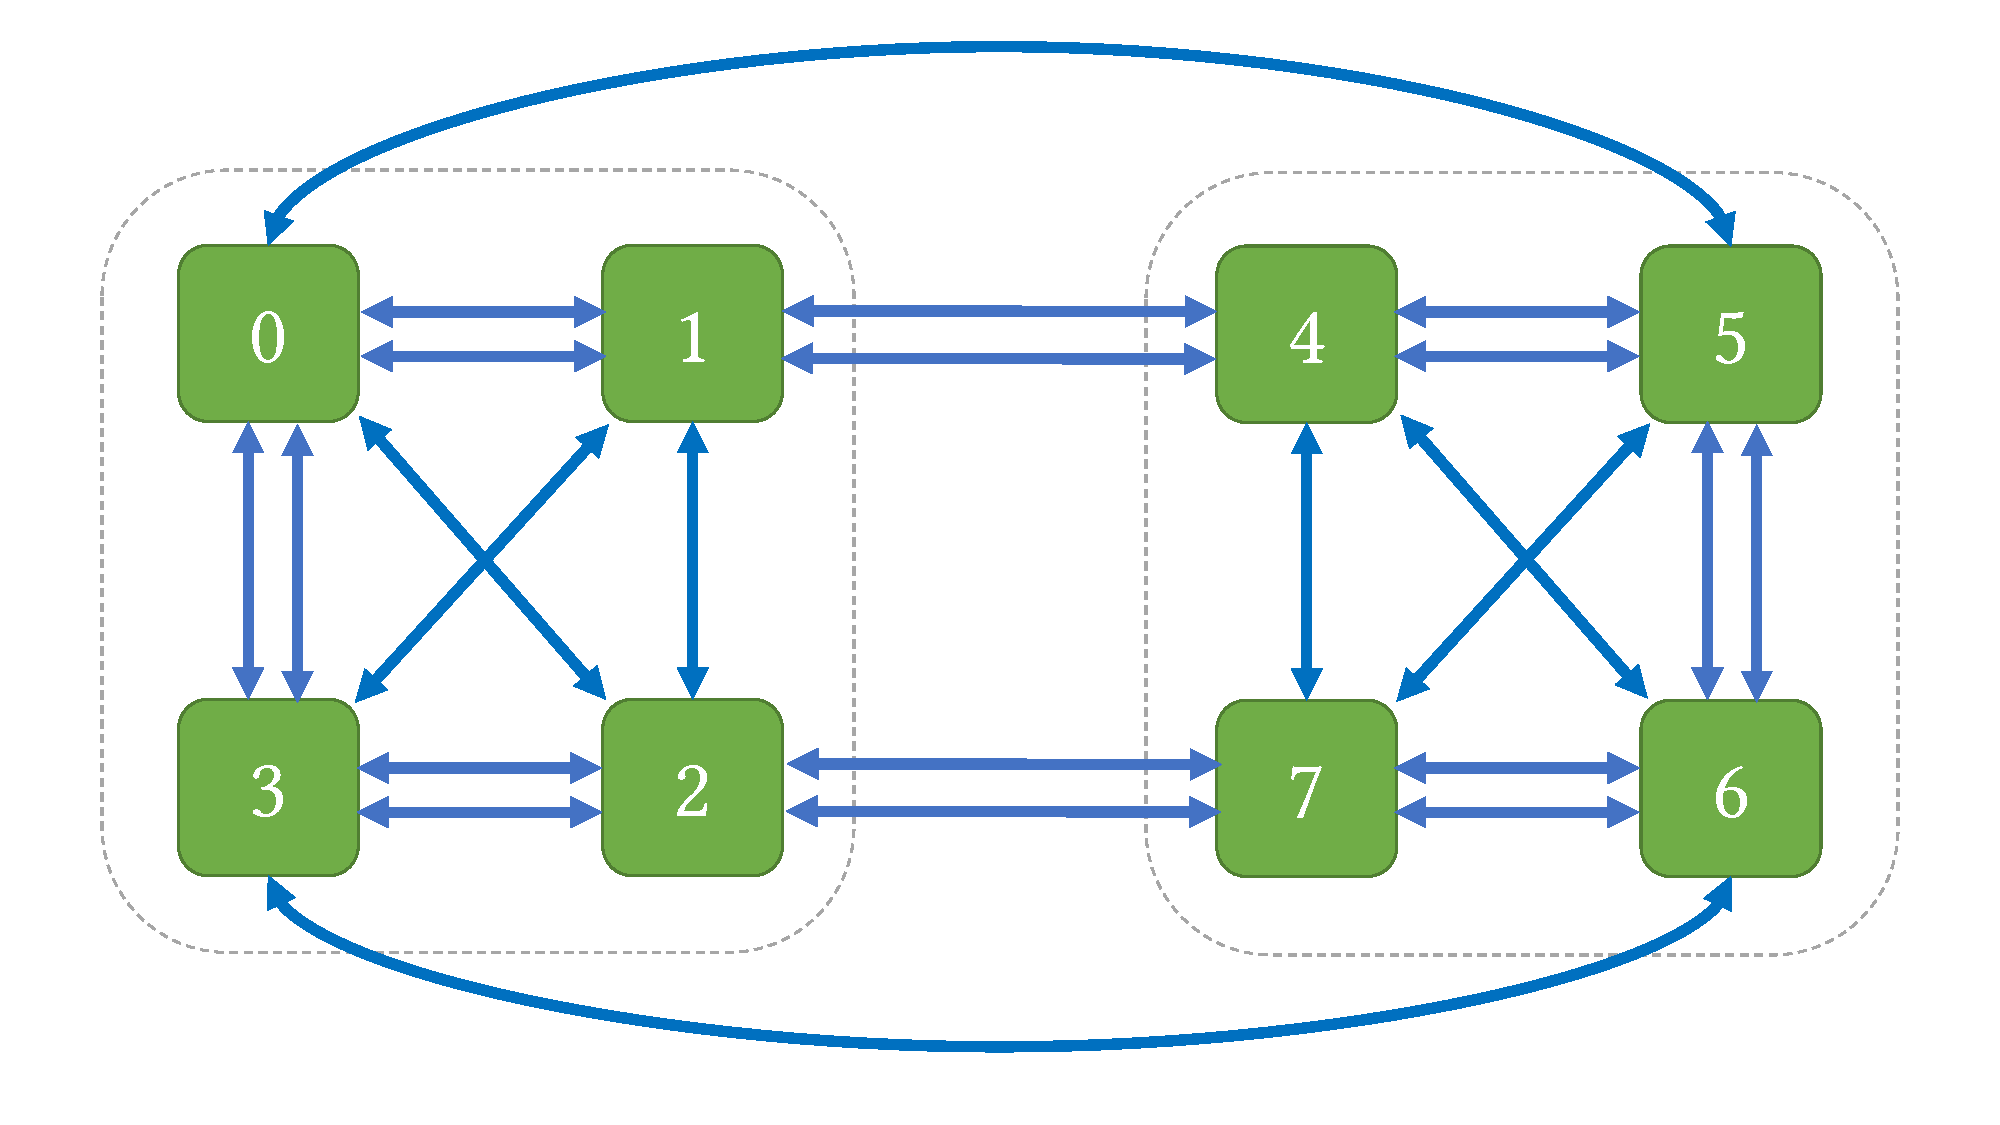
\includegraphics[page=1,width=\columnwidth]{figures/topos.pdf}
\caption{NVLink topology of an NVIDIA DGX-1.}
\label{fig:dgx1-topo}
\end{figure}
%\todo{the grey box indicating a socket has a low contrast when printed. colours for two different rings should have higher contrast (blue and orange perhaps?)}

% explain our approach
In this chapter, we automatically synthesize high-performance communication kernels.
Given a topology, specified as a graph with bandwidth constraints on nodes and edges, and a communication primitive, specified as the pre- and post-condition on data location and computation on it, we generate~(Section~\ref{sec:synthesis}) a quantifier-free SMT formula that captures the set of all feasible algorithms that implement the primitive on the input topology.
Exploring this space to appropriately minimize the number of communication steps or decrease the granularity of communication at each step, is a computationally difficult problem. We exploit
an SMT solver to synthesize algorithms that explore this tradeoff along the Pareto frontier between latency-optimality and bandwidth-optimality.
For every solution from the SMT solver, we automatically generate and lower~(Section~\ref{sec:lowering}) high-performance implementations.


% We approach this problem as a synthesis problem. Collective communication
% primitives can be specified in terms of pre- and post-conditions on which
% processes data resides on and optionally where a user specified reduction
% function has been applied. We encode pre- and post-conditions as well as actions
% to move data between processes as quantifier-free SMT formulas, which we solve
% using Z3. We further impose constraints on bandwidth usage based on the topology
% of the specific machine we are targeting and limit the number of steps for the
% whole algorithm. This gives us a way to explore the entire space of possible
% algorithms for implementing a given primitive on the target hardware.

% how do we make it scalable
When using SMT, finding the right encoding can make all the difference for the
feasibility of an approach. This paper details the important design choices in
our encoding that help it scale to all of our hardware targets. We use the SMT
encoding for \broadcasting collectives, such as \broadcast, while for \reducing
collectives, such as \reduce, we employ a reduction back to the synthesis
problem for \broadcasting collectives.
%A key observation is that topologies have natural symmetries. Our encoding exploits this symmetry to efficiently explore the space of algorithms without sacrificing satisfiability.
This reduction generalizes a well known fact that some \reducing collectives may
be produced by inverting a \broadcasting one, e.g. \reduce by inverting \broadcast.

%This allows us to reuse
%the synthesis of certain primitives such as \allreduce, further improving our
%scalability.
%\todo{"time time-reversed mirror-image", huh? find easier to understand wording.}
%\todo{what do you mean by "modularize"? it's more like we reduce (no pun intended) the problem of reduction to broadcasting, which is the wording used later in bullet points}

% This informed an optimization in
% our encoding, that allows us to make reasoning about which GPUs data has been
% reduced implicit.

%\todo{This is quite vague right now.}

% The ability to control the number of steps an algorithm must execute in gives us
% a novel capability for trading off between latency and bandwidth optimality. By
% synthesizing a range of algorithms at different points in this space we can use
% the best algorithm for any given message size. While MPI implementations and
% NCCL both switch between algorithms based on message size, our synthesis
% approach allows us to do so in a much more fine grained manner. We show that
% this enables our algorithms to provide better performance than NCCL at all
% message sizes. \todo{Update this claim with truth.}

We implement our approach in a tool called \toollong{}~(\tool{}),
which probes the target hardware topology, synthesizes algorithms for
it using Z3~\cite{z3} and finally generates CUDA code that efficiently implements that algorithm.  These algorithms are
synchronous; at every step of the algorithm, one or more of the nodes
send and/or reduce data from others.
%\todo{"CUDA code"=>hardware dependent code? we have AMD GPUs. From saemal: AMD runs CUDA. OpenCL is another possibility but no one really uses it.}

% algorithmic novelty
Some of the algorithms we synthesize are novel, with no known counterparts in
the literature occupying the same latency-bandwidth tradeoff. For example, we
have produced a latency-optimal 2-step (4-step) algorithm for
the \allgather (\allreduce) primitive in the DGX-1 topology (Figure~\ref{fig:dgx1-topo}) and
a bandwidth-optimal 3-step (6-step) algorithm for the \allgather (\allreduce) primitive on the
same topology.  In addition to providing novel
algorithms, our approach informs us when a combination of bandwidth and number
of steps is \emph{not possible}. This makes our synthesis approach a tool for
probing the algorithmic properties that a given topology provides, which is
useful for co-design of hardware interconnects with communication libraries.
%\todo{"occupying the same latency-bandwidth tradeoff": exhibiting? and being different isn't necessarily good, we want more bandwidth with the same latency or lower latency with the same bandwidth.}
%\todo{tell reader that the "number of steps" correlate with latency?}
% results
Our evaluation~(Section~\ref{sec:evaluation}) shows us that this approach scales and beats NCCL in almost all cases.


To summarize, the contributions of this chapter are as follows:
\begin{itemize}
    \item A formalization of the synthesis problem for \broadcasting collectives.
    \item A general strategy for encoding the synthesis problem for
    collective communications algorithms into the quantifier-free linear integer
    arithmetic (QF\_LIA) sub-logic of the SMT-LIB logic.
    \item A reduction from the synthesis problem for \reducing collectives to that for \broadcasting collectives.
    % \item Explanations of some novel algorithms our synthesis has produced.
    \item A description of how \tool{} generates efficient code for the algorithms we synthesize on nodes with NVIDIA or AMD GPUs.
    \item An evaluation of \tool's generated algorithms on common server topologies for deep learning workloads and a comparison against NCCL.
\end{itemize}

%\todo{Paper structure paragraph?}

%%% Local Variables:
%%% mode: latex
%%% TeX-master: "paper"
%%% End:

\section{Overview}
This section provides an overview of synthesizing latency- and bandwidth-optimal algorithms, using \allgather for the
\dgxone topology~(Figure~\ref{fig:dgx1-topo}) as the running example.

\subsection{Collective Communication Primitives}
\label{sec:background-collectives}
Collective communication primitives allow nodes in a networked system to perform operations on shared data. As an example, if each node has some input data, the \allgather primitive transfers these data to all of the nodes.  One way to implement this is for each node to independently send its data to all other nodes. But, an algorithm in which the nodes collectively work together can be more efficient. The efficiency of such algorithms depends on the network topology.

\begin{comment}
    For instance, given a set of nodes each having an array of data, the \allreduce primitive computes the sum (or some specified associative operation) of all these arrays and stores the result in each of these arrays.

Computing the primitives such as \allreduce requires the nodes to communicate. This communication usually happens in smaller chunks of the input array. Given $N$ nodes, say we split the input array into $N$ chunks, where $c_{i,j}$ represents the $i$th chunk at node $j$. One way to compute \allreduce is as follows. First, we compute at node $i$, a partial sum $d_i = \sum_j c_{i,j}$. These reductions can be performed by arranging $N$ nodes in a spanning tree and communicating chunks $c_{i,j}$ along the tree. Note, there are $N$ parallel reductions each possibly using a different spanning tree. This arrangement of reduced data is called the \reducescatter primitive. Once we have the chunks $d_i$, we can perform an \allgather operation by ensuring each node has a copy of $d_i$. In essence, \allgather involves $N$ simultaneous broadcasts of $d_i$ from node $i$. Thus, we have implemented \allreduce by performing an \reducescatter followed by an \allgather.
\todo{I think the ``$N$ parallel reductions each possibly using a different spanning tree'' makes this confusing---is this describing an approach where each node reduces $1/N$ of the chunks?}
\todo{say "compute at node $i$, a partial sum" of chunk $i$.}
\todo{they're are a part of the sum of arrays. they are not really partial sums, in the sense that, e.g., only data from half of the nodes are added.}
\todo{"there are $N$ parallel reductions"=>these $N$ parallel reductions}

Implementing a collective communication primitive depends on the topology. For instance, when executing parallel reductions or broadcasts in the implementation above, the algorithm has to choose different spanning trees to utilize the bandwidth on all links in the topology. Similarly, the algorithm has to choose the ideal chunk size to use for communication. We will demonstrate these choices for the \dgxone topology described below.
\todo{"Implementing" $\ldots$ efficiently}
\todo{"has to chose ": might have to choose}
\end{comment}

\subsection{Topology}
The network topology specifies how the nodes are connected with each other and the latency and bandwidth constraints on the links connecting them. Consider the \dgxone topology shown in Figure~\ref{fig:dgx1-topo}. It consists of $8$ GPUs (or nodes, in the above formalism) split into two groups $\{0,1,2,3\}$ and $\{4,5,6,7\}$. The nodes in each group are fully connected. In addition, there are four inter-group links as shown in the figure. These nodes are connected through
NVLinks, with some nodes connected with two parallel NVLinks as shown in Figure~\ref{fig:dgx1-topo}.

%There are two kinds of links shown in two different colors. The fast links, such as the one connecting nodes $0$ and $1$ have twice the bandwidth as the (relatively) slow links, such as the one connecting nodes $0$ and $2$. The figure represents the fast links with two arrows. Each link is bidirectional allowing concurrent sends and receives at full bandwidth.
%\todo{Remove the colors and the double arrow should make it clear}
%\todo{Also just mention that they are called nv2 and nv1 links}
%\todo{"split into two" groups, each associated with one CPU socket.}
%\todo{"All the nodes within a socket": all the GPUs in the same group}
%\todo{"inter-socket links" sound like QPI: maybe inter-group?}
%\todo{also check the usage in latency-optimal algorithm}
%\todo{I recommend talking about these in terms of groups rather than sockets to avoid the NVLink/PCIe/QPI confusion too -jn}
%\todo{I also recommend not talking about ``fast'' and ``slow'' links, since the diagram shows a fast link as 2 slow links (which is indeed what it is), and we then talk about using 6 logical rings; better to just say 6 links and 6 rings}

The \dgxone's design was heavily influenced by the need to do gradient reduction for machine learning workloads. Specifically, this topology forms two non-overlapping rings: one connecting nodes $\{0,1,4,5,6,7,2,3\}$ with two NVLinks per edge and another connecting $\{0,2,1,3,6,4,7,5\}$ with one NVLink per edge. These rings are bidirectional and thus form $6$ logical single-NVLink rings. The NCCL library implements \allgather by running $6$ simultaneous ring algorithms as we discuss below.

%Given the fast ring has twice the bandwidth and each ring is bidirectional, this allows the implementation to utilize $6$ logical rings with the same bandwidth %to implement collection primitives
%(2 from the slow ring and 4 from the fast ring).

\subsection{Cost Model}
%\todo{I think we need to define bandwidth and latency optimality here. My understanding is that a bandwidth-optimal algorithm is one that sends the minimal amount of data necessary to complete its operation, and a latency-optimal one uses the fewest number of communication rounds possible to complete its operation. Is that what we mean?}

%Before discussing how to build bandwidth- and latency-optimal algorithms for this topology, we will introduce a simple cost model.
We will characterize the communication cost using the $(\alpha, \beta)$ model~\cite{hockney1994communication}. That is, sending a message of size $L$ along a link costs $\alpha + L\cdot\beta$ time.
Here, $\alpha$ is the latency of communication and captures the {\em fixed} costs, such as the overhead of initiating a transfer or invoking a GPU kernel,
and $\beta$ is the inverse bandwidth of the link and captures {\em per-byte} costs, such as copying data into system buffers. Li \etal{} extensively studies the transfer time of buffers with
different sizes over numerous GPU interconnections\cite{alphabeta}. Their result show that with NVLinks, the transfer time stays almost constant up-to a large buffer size and only then it start to increase linearly.
These results confirm that the $(\alpha,\beta)$ model is suitable for characterizing communication cost over NVLinks.

The cost of a collective algorithm for an input of size $L$ will be of the form $a\cdot\alpha + b \cdot L \cdot \beta$. We call $a$ the {\em latency cost} of the algorithm and $b$ the {\em bandwidth cost} of the algorithm. Given a class of algorithms that implement a collective on a given topology, an algorithm is {\em latency-optimal} ({\em bandwidth-optimal}) if no other algorithm in the class has a lower latency (bandwidth) cost. Usually, there is a tradeoff between the latency cost and the bandwidth cost when designing collective algorithms.  An algorithm with latency cost $a$ and bandwidth cost $b$ is said to be {\em Pareto-optimal} with respect to a class of algorithms if for every algorithm in the class with latency cost $a'$ and bandwidth cost $b'$, we have $a = a' \Rightarrow b' \geq b$ and $b = b' \Rightarrow  a' \geq a$.

%The $\alpha$ term represents the {\em fixed} cost of sending a message from the overhead of invoking a GPU kernel to the latency across the network. The $beta$ term represents from the cost of copying data across system buffers to the time taken to transmit the bytes at a given network bandwidth. For small message sizes, the cost is determined by the fixed cost $\alpha$, while for large message sizes, the cost is determined by the per-byte cost $\beta$.
%\todo{we are going to have a single kernel launch, so many not the kernel launch cost?}
%\todo{give our estimation of $\alpha$ and $\beta$ cost for DGX1 and NVLinks.}
%\todo{the from $\ldots$ to $\ldots$ in a long sentence is confusing: consider "such as"}
%\todo{note: I replaced ``packet'' with ``message'', since alpha is more about the cost to initiate a transfer rather than to send a single 256-byte NVLink packet}

\subsection{Bandwidth-Optimal Algorithm for \dgxone}
\label{sec:motivation:bw-optimal}
As described above, the \dgxone topology has $6$ logical rings. \allgather for one ring can be implemented as follows. Each node simultaneously sends its data to the next node in the ring. In subsequent steps, each node stores the received data and sends it to the next node in the ring. In $7$ steps all nodes will have received data from all of the other $7$ GPUs. The $6$-ring algorithm is a generalization of this algorithm. Each node splits its data into $6$ chunks and executes the ring algorithm along each of the $6$ rings, with one chunk per ring. If $L$ is the size of the input data, each ring algorithm takes $7$ steps and communicates $\frac{L}{6}$ bytes. Thus, the cost of the $6$-ring algorithm is
$$7\cdot \alpha + \frac{7}{6}\cdot L \cdot \beta$$

Each node has to receive at least $7 \cdot L$ amount of data, and it has an agglomerated incoming per-byte cost of $\beta/6$ (6 incoming NVLinks). Thus, any algorithm for \allgather has to take at least $\frac{7}{6}\cdot L \cdot \beta$ amount of time. Thus, this algorithm is bandwidth-optimal for the \dgxone topology. But can we do better with the latency cost?

Using the techniques described in this paper, we have automatically synthesized an algorithm~(Section~\ref{fig:dgxone:syn}) with cost $$3\cdot \alpha + \frac{7}{6}\cdot L \cdot \beta$$ To the best of our knowledge, this algorithm was not previously known. Moreover, we prove that this algorithm is Pareto-optimal with respect to the class of algorithms we call $k$-synchronous algorithms~(Section~\ref{sec:ksync}).

\subsection{Latency-Optimal Algorithm for \dgxone}
The next question is whether we can improve upon the latency cost of the synthesized algorithm. If each node communicates its data along a binary tree instead of a ring, it would take at least $3$ steps. Using the techniques described in this paper, we have automatically synthesized a better algorithm~(Section~\ref{fig:dgxone:syn}) with cost $$2\cdot \alpha + \frac{3}{2}\cdot L \cdot \beta$$
Since the \dgxone topology has a diameter of $2$, this algorithm is latency-optimal. To the best of our knowledge, a latency-optimal algorithm for the \dgxone was not previously known. This algorithm is Pareto-optimal with respect to the class of $k$-synchronous algorithms.

\begin{comment}
While bandwidth optimal algorithms are suitable for large inputs $D \gg \alpha / \beta$, they are wasteful for small inputs. In such cases, we seek a latency-optimal algorithm. NCCL is
capable of creating trees but on a \dgxone, the created trees are always a line graph and
therefore, they have the same latency as a ring.
\todofor{Saeed}{Does NCCL have a tree based allgather? If not, what's the tree like in allreduce? Is it binary? from saemal: no it does not. For allgather it doesn't even have
any other implementation other than a ring and for allreduce on DGX1, it only creates a ring with the tree. It is safe to say that on DGX-1 they use a ring always even though they have the capability of doing a tree}
\todo{"they are wasteful for small inputs"=>they might not give the smallest possible latency for small inputs}

The technique discussed in this paper synthesized a better algorithm that takes $2$ steps! To the best of our knowledge, this algorithm is not previously known. The algorithm works as follows. In the first step, each node sends its chunk to all its neighbors. For instance, node $0$ sends its chunk to its intra-socket neighbors $1$, $2$, and $3$ as well to its inter-socket neighbor $5$. Since each link is bidirectional communication from nodes do not conflict. At the end of step 1, each node has received chunks from all its intra-socket neighbors and one chunk from its inter-socket neighbor. In the second step, each node sends the chunk from its inter-socket neighbor to all its intra-socket neighbors. That is, node $0$ sends the chunk from $5$ to nodes $1$, $2$, $3$.

This two-step algorithm does not subdivide its input data of size $D$. So, we will call this algorithm a \chunkstep{1}{2} algorithm. The time taken by this algorithm is
$$2\cdot \alpha + 2\cdot D\cdot\beta$$
Since the diameter of this topology is $2$ and each node has to communicate with every other node, one cannot implement an \allgather in one step. Thus, for $D \ll \alpha / \beta$, this algorithm is optimal. We call such algorithms latency optimal.

A natural question, again, is whether a faster latency optimal algorithms exist that can use the bandwidth more efficiently. For instance, the \chunkstep{1}{2} does not make use of fast bandwidth links as it only sends one chunk between a pair of nodes at each step. This paper shows that such an algorithm exist.
\todo{Not true, with rounds, we have a better algorithm.}

\subsection{Pareto Frontier}
\label{sec:pareto}

While the bandwidth-optimal algorithm is suitable for large input sizes and the latency-optimal algorithm is for small input sizes, many interesting inputs might be of sizes in between the two limits. How do design optimal algorithms in such cases? Let us assume that a \chunkstep{c}{s} algorithm implementing a collective on a given topology exists. Using a similar reasoning as above, this algorithm will take time
$$ s\cdot \alpha + \frac{s\cdot D \cdot \beta}{c}$$
Intuitively, we need to reduce $s$ to improve the latency of the algorithm and increase $c$ to improve the bandwidth utilization of the algorithm, while the constraints of the topology and the implemented collective will restrict the feasible pairs $(c,s)$. For instance, as argued above, $s \geq 2$ and $\frac{s}{c} \geq \frac{7}{6}$ when implementing \allgather on the \dgxone topology. In other words, for a given $s$, $c \leq \left\lfloor\frac{6 \cdot s}{7} \right\rfloor$.
\todo{maybe need to justify why all algorithms can be expressed as \chunkstep{c}{s} performance-wise. Suppose different ranks have different number of steps, which takes different durations. Even though you can find the smallest time slice and the corresponding greatest common divisor logical chunk size, the steps now are "logical" steps, and you don't always pay the $\alpha$ cost.}
\todo{our algorithms are BSP. With the concept of rounds, each step might take different amount
of time. Since 1 bw and 2 bw have 2 as their lcm, having equal chunks makes sense. Maybe we should have this in Section 2?}


By trading latency by increasing $s$, one can search for the largest $c$ for which a feasible \chunkstep{c}{s} exists. Each such algorithm maximizes the bandwidth utilization for a given latency. We can increase $s$ till we reach a bandwidth-optimal algorithm. Together, these form a {\em Pareto frontier} of feasible algorithms. Which of these algorithms to use will depend on the size of the input data $D$, the latency $\alpha$ of the network, and the bandwidth $\beta$ of the network.

\subsection{Summary of the Paper}
In this paper, we propose a systematic method to synthesize algorithms in the Pareto-frontier spanning form the latency-optimal algorithm to the bandwidth-optimal algorithm for a given collective on an input topology. We characterize a class of algorithms that captures a broad set of known algorithms and prove Pareto-optimality of both known algorithms and synthesized new algorithms. We automatically generate an implementation of these algorithms that is competitive with manually hand-tuned communication kernels in use today.

\end{comment}


%\subsection{Synthesizing Optimal Algorithms}
%\todofor{Olli}{Summarize our approach to synthesizing algorithms on the pareto frontier.}
%Given a topology, we automatically optimal algorithms in the pareto frontier.  Essentially a summary of the paper.

\section{Algorithm Synthesis}
\label{sec:synthesis}
This section demonstrates a method to synthesize Pareto-optimal
algorithms that implement a collective primitive on a given topology.
The Pareto-optimality is defined with respect to a class of algorithms
we call {\em $k$-synchronous} algorithms.

We distinguish between {\em \reducing} collectives such as \allreduce
and \reducescatter that combine chunks through computation, and {\em
\broadcasting} collectives such as \allgather and \broadcast that
simply transfer data among nodes. We will focus on synthesizing
\broadcasting collectives and show how to derive \reducing collectives
from related \broadcasting ones.

\subsection{$k$-synchronous Algorithms}
\label{sec:ksync}
%automation.
\begin{figure}
    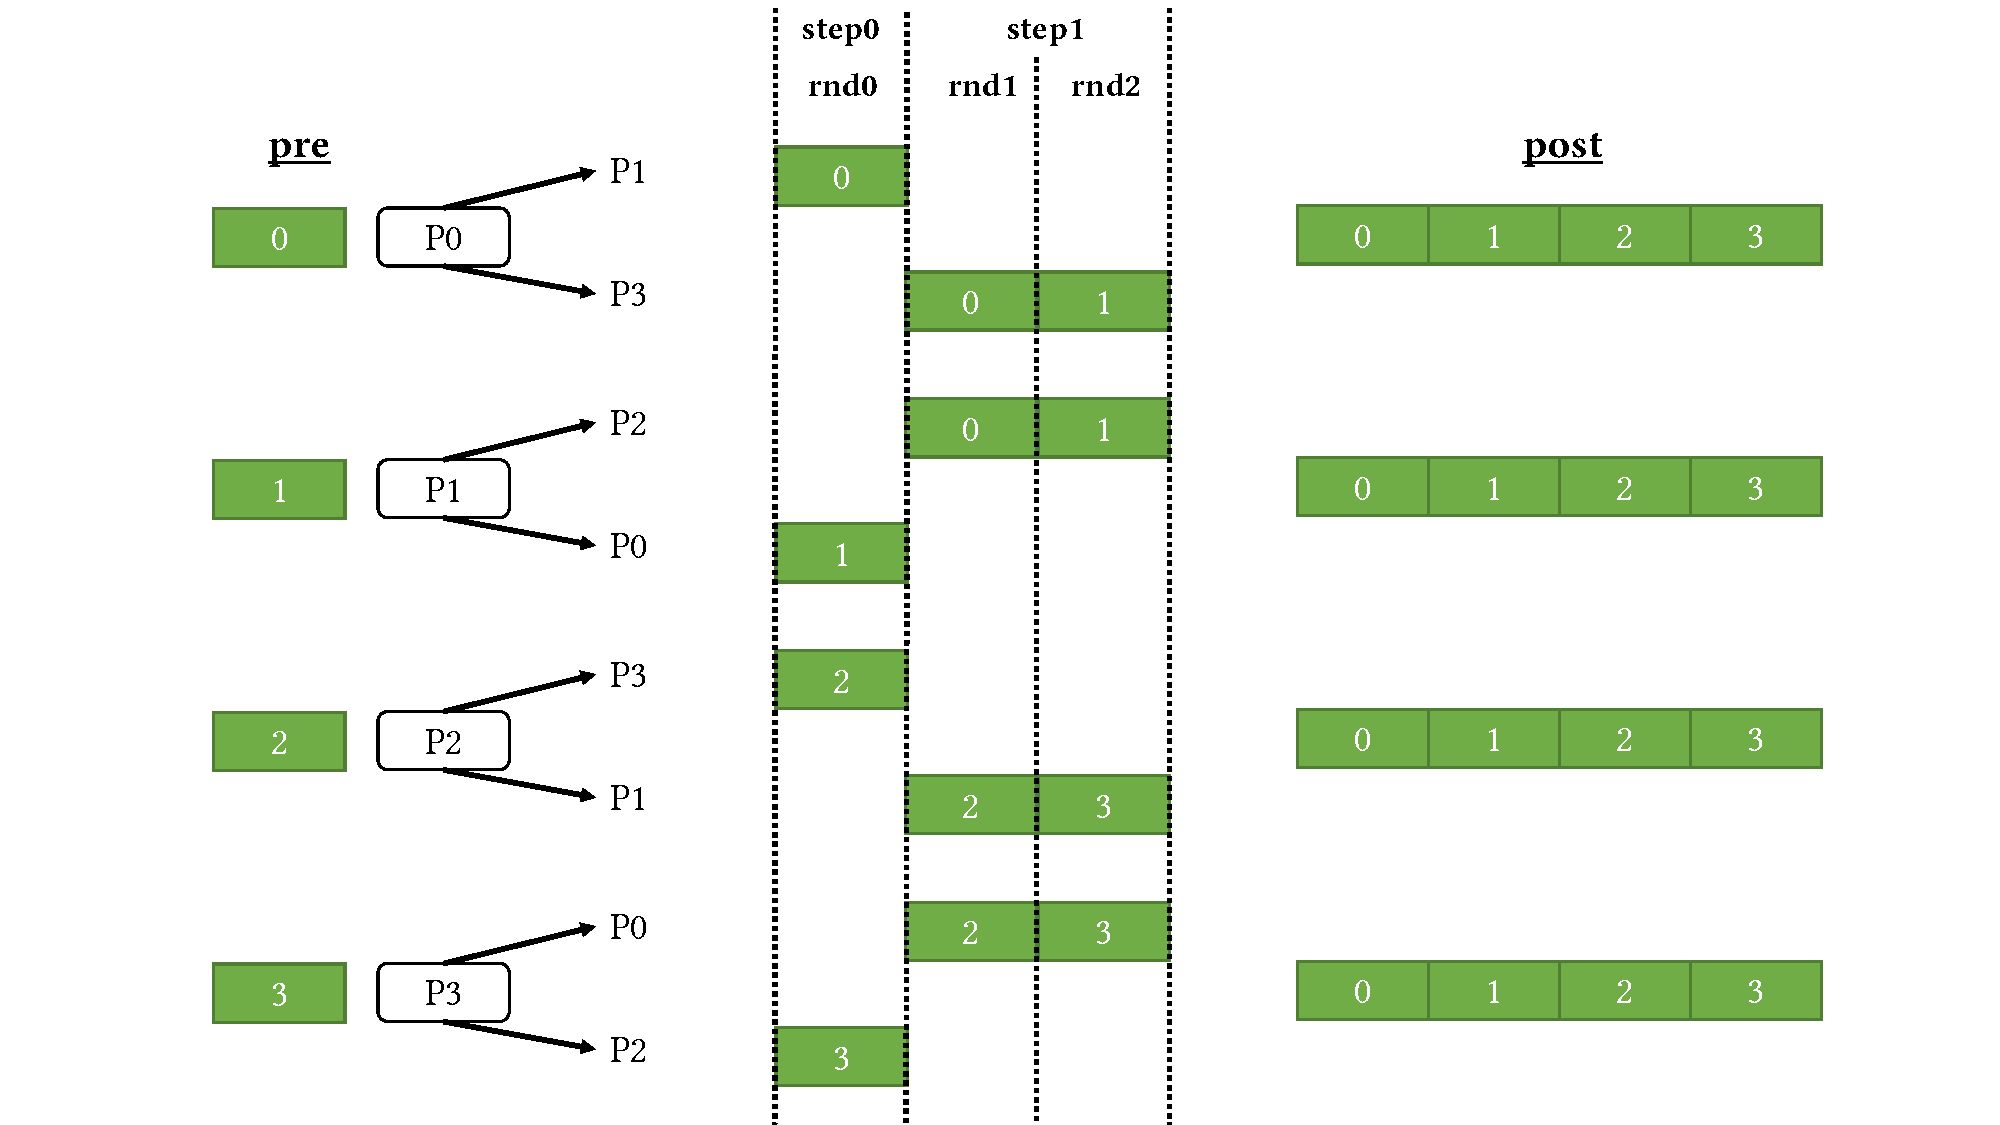
\includegraphics[width=\columnwidth]{figures/allgatherex.pdf}
    \caption{A $1$-synchronous algorithm for \allgather on a ring topology.}
    \label{fig:allgatherex}
\end{figure}

Figure~\ref{fig:allgatherex} shows the
recursive-doubling~\cite{thakur2005optimization} algorithm for
\allgather for a ring topology of four nodes $P0, P1, P2, P3$ with
four bidirectional links of equal bandwidth. This algorithm proceeds
in two {\em steps}. In the first step, nodes at "distance" 1, namely
$P0, P1$ and $P2, P3$ send their data to each other. Each node now has
data from two nodes, which it communicates entirely with nodes at
distance 2, i.e., nodes $P0, P3$ and $P1, P2$ in the second step. At
the end, each node has data from every other node. Since the second
step involves sending twice the amount of data as the first step, we
say it has two \emph{rounds} where in each round, it sends data. Thus,
this step has a total of $3$ rounds. Of the eight (unidirectional)
links, this algorithm uses only four of them per step. To improve
bandwidth utilization, a better option is to split the input data into
equal-sized {\em chunks} and communicate them independently. For
instance, the ring algorithm described in
Section~\ref{sec:motivation:bw-optimal} uses $3$ chunks per node.

The algorithm in Figure~\ref{fig:allgatherex} and many classical
collective algorithms~\cite{thakur2005optimization,chan2007collective}
are instances of {\em synchronous} algorithms. A synchronous algorithm
proceeds in a sequence of synchronous communication {\em steps} with
nodes waiting for other nodes to finish their rounds before starting
the next step. Even if an implementation might not enforce a global
barrier across the nodes, these algorithms choose the amount of data
to communicate per step based on the bandwidth constraints so that the
nodes finish each step at (roughly) the same time.

Many algorithms, like the one in Figure~\ref{fig:allgatherex},
communicate different numbers of chunks per step. We consider each
step as consisting of multiple rounds with each node sending at most
one chunk per unit-bandwidth on its outgoing links. Intuitively, the
number of rounds in an algorithm controls its bandwidth cost, while
the number of steps controls its latency cost. A synchronous algorithm
with $\steps$ steps and $\rounds$ rounds is {\em $k$-synchronous} if
$\rounds \leq \steps + k$. The parameter $k$ limits the amount of
communication per step and allows an SMT solver to effectively search
the space of algorithms bounded by that $k$.
%\todo{Madan mentioned in the chat that for a given $k$, we use it to
%bound $R$. We can make it clearer. The first time I read this, I
%thought we are changing $k$ for some $R$ and $S$ such that $k$ is the
%smallest number such that $R\le S+k$.}

%The terminology of steps and rounds might be confusing at first. The
%best way to distinguish them is to note that in the $(\alpha, \beta)$
%cost model, the latency cost of a $k$-synchronous algorithm depends
%on the number of steps, while the bandwidth cost depends on the
%number of rounds and the number of the chunks.

\subsection{\broadcastingCap Collective Instance}
Now we will provide a uniform formulation for representing
$k$-synchronous algorithms for \broadcasting collectives. An instance
of \collectiveproblem is a tuple
$(\gchunk,\steps,\rounds,\size,\bw,\pre,\post)$, where
\begin{itemize}
    \item[] \hspace{-0.5cm}Parameters:
    \begin{itemize}
    \item $\gchunk\in\posint$ is the global number of chunks
    \item $\steps\in\posint$ is the total number of steps
    \item $\rounds\in\posint$ is the total number of rounds
    \end{itemize}
    \item[] \hspace{-0.5cm}Topology:
    \begin{itemize}
    \item $\size\in\posint$ is the number of nodes
    \item
    $\bw\subseteq\powerset(\range{\size}\times\range{\size})\times\mathbb{N}$
    is the bandwidth relation
    \end{itemize}
    \item[] \hspace{-0.5cm} Specification:
    \begin{itemize}
        \item $\pre\subseteq\range{\gchunk}\times\range{\size}$ is the
        pre-condition
        \item $\post\subseteq\range{\gchunk}\times\range{\size}$ is
        the post-condition
    \end{itemize}
\end{itemize}
Note that for a set $M$ we write $\powerset(M)$ for the power set of
$M$, i.e., the set of all subsets. For an integer $x$, we write
$\range{x}$ for the set $\{0, 1, \ldots, x\}$. Here, $\gchunk, \steps,
\rounds$ are parameters to the desired $k$-synchronous algorithm. The
rest are explained below.

\subsubsection{Topology}
\label{sec:topology}
$\size$ is the number of nodes in the topology. $\bw$ gives a flexible
way to express different bandwidth constraints we have seen in
practice. In its most general form, $\bw$ bounds the sum of chunks
sent along a set of edges in a single round. A point-to-point
communication link from $s$ to $d$ with maximum bandwidth (in chunks
per round) $b$ can be modeled by $(\{(s, d)\}, b) \in \bw$. Some
topologies might limit the net outgoing bandwidth $b$ from a certain
node $s$. If $E$ is the set of outgoing neighbors of $s$, we can model
this by $(\{(s, e) \mid e \in E\}, b) \in \bw$. To model shared bus
topologies, where only one node can send in a round, we include
$(\{(a, b) \mid a \in N, b \in N\}, b)$ in $\bw$ for the set of nodes
$N$ sharing the same link. Note that these constraints are per round,
and when performing $r_i$ rounds in step $i$, we simply multiply the
bandwidth constraint by $r_i$.

\newcommand{\relAll}{All\xspace}
\newcommand{\relRoot}{Root\xspace}
\newcommand{\relScattered}{Scattered\xspace}
\newcommand{\relTranspose}{Transpose\xspace}
\newcommand{\chunkReduce}{\left\lfloor\frac{i}{\size}\right\rfloor}
\begin{table}
    \center
    \begin{tabularx}{\columnwidth}{@{}Xl@{}}
        \toprule
        Name & Relation \\
        \midrule
        \relAll & $\range{\gchunk}\times\range{\size}$ \\
        \relRoot & $\range{\gchunk}\times\{n_\mathit{root}\}$ \\
        \relScattered & $\{(c,n)\in\range{\gchunk}\times\range{\size}
        \setwhere n=c\bmod \size\}$ \\
        \relTranspose & $\{(c,n)\in\range{\gchunk}\times\range{\size}
        \setwhere n=\left\lfloor\frac{c}{\size}\right\rfloor\bmod
        \size\}$ \\
        \bottomrule
    \end{tabularx}
    \caption{Common relations in pre- and post-conditions of collective primitives.}
    \label{tbl:relations}
\end{table}
\begin{table}
    \begin{tabularx}{\columnwidth}{@{}Xll@{}}
        \toprule
        Collective & $\pre$ & $\post$ \\
        \midrule
        \gathercoll & \relScattered & \relRoot  \\
        \allgather & \relScattered & \relAll  \\
        \alltoall & \relScattered & \relTranspose  \\
        \broadcast & \relRoot & \relAll \\
        \scatter & \relRoot & \relScattered  \\
        \bottomrule
    \end{tabularx}
    \caption{Specifications of collective primitives.}
    \label{tbl:collectives}
\end{table}

\begin{comment}
    \begin{table}
    \begin{tabularx}{\columnwidth}{@{}Xlll@{}}
        \toprule
        Collective & $\pre$ & $\post$ & $\chunk(c)$ \\
        \midrule
        \gathercoll & \relScattered & \relRoot & $c$ \\
        \allgather & \relScattered & \relAll & $c$ \\
        \alltoall & \relScattered & \relTranspose & $c$ \\
        \broadcast & \relRoot & \relAll & $c$ \\
        \scatter & \relRoot & \relScattered & $c$ \\
        \reduce & \relScattered & \relRoot & $\chunkReduce$ \\[2pt] %
        make sure floor symbols don't stick together
        \allreduce & \relScattered & \relAll & $\chunkReduce$ \\[2pt]
        \reducescatter & \relScattered & \relTranspose &
        $\chunkReduce$ \\[2pt]
        \bottomrule
    \end{tabularx}
    \caption{Specifications of collective primitives as \collectiveproblem instances using a small set of common relations for pre- and post-conditions.}
    \label{tbl:collectives}
\end{table}
\end{comment}
\subsubsection{Collective Specification}
\label{sec:specifications}
The $\pre$ relation specifies the nodes where the chunks reside at the
beginning of the algorithm and the $\post$ relation specifies the set
of nodes where a chunk needs to be transferred to.
Table~\ref{tbl:relations} specifies useful relations that can be used
to specify common collectives as shown in Table~\ref{tbl:collectives}.
For instance, \allgather starts in a state where chunks are in the
\relScattered relation in Table~\ref{tbl:relations}. In other words,
the $c$ chunks of the input at node $n$ are given chunk identifier
$i\cdot P + n$ for $0 \leq i < c$. From this \relScattered state,
\allgather requires all the input chunks to be copied to all nodes, as
specified by \relAll relation in Table~\ref{tbl:relations}. Similarly,
\broadcast requires all the chunks from the root $n_{root}$ to be
copied to all nodes.

\begin{comment}
We have identified a small number of relations
(Table~\ref{tbl:relations}) that can be mixed-and-matched to model
most common collective primitives (Table~\ref{tbl:collectives}).
Collectives using \relRoot require that a root node $n_\mathit{root}$
has been given. The \relScattered relation is used in collectives that
evenly distribute input data onto nodes, and collectives that use it
require that $\chunk\bmod\size=0$ The \relTranspose relation is used
in conjunction with \relScattered to re-distribute scattered data, and
to ensure an even redistribution these collectives require that
$\chunk\bmod\size^2=0$.

\allreduce as it is specified in Table~\ref{tbl:collectives} needs an
associative reduction operation or else it can give different results
on different nodes. See Section~\ref{sec:background-collectives} for
more discussion.
\todo{Point this Section reference to where the allreduce discussion actually ends up at.}
\end{comment}

\begin{comment}
nodes each identifier starts from, while $\post$ specifies the nodes
that each identifier must end up on. For example, a point-to-point
send primitive with $\size=2$ and $\chunk=1$ might have
$\pre=\{(0,0)\}$ and $\post=\{(0,1)\}$. Note that the pre-condition
can specify that copies of an identifier start from multiple nodes,
which is not useful for traditional collectives. However, this feature
can be useful for specifying more exotic collectives for situations
where an application has already placed identical copies of data onto
some nodes.
\end{comment}

\begin{comment}
% Madan moved this to earlier

The bandwidth relation $\bw$ gives a flexible way to express various
kinds of networks. Topologies with direct links between a source node
$s$ and a destination node $d$ will have $\bw$ of the form
$\{(\{(s,d)\},b),(\{(s',d')\},b'),\dotscend\}$, where $b,b',\dotscend$
give the per link bandwidths. And, to limit the total outgoing
bandwidth from a node $n$ to be no more than $b$, may be modeled with
an entry of the form $(\{(n,n') \setwhere n'\in\range{\size}\},b)$. A
switch that all traffic between two sets of nodes $P$ and $Q$ can be
modeled with an entry of the form $(\{(n,n') \setwhere n\in P \wedge
n'\in Q\},b)$. See Section~\ref{sec:topologies} for details on how we
model the network topologies found in our hardware targets.
\end{comment}

\begin{comment}
The qouta relation $\qouta$ allows multiple chunks be sent in a step
through a link. A link with a bandwidth of $b$ can transfer $2b$
chunks in a 2 short steps which each transferring $b$ chunks but
alternatively the same link could transfer $2b$ chunks in a longer
step. This enables the synthesizer to find algorithm which are more
latency optimal.
\todofor{Olli}{Do we want to talk about sharing of nodes here? - this is important as most cross node topologies have shared interconnects in addition to PCIe}
\todofor{Olli}{our assumptions below  do not allow different sized chunks.  this is fine, but i wonder if we want to have a section on our ``asusmptions'' to push off potential challenges from reviewers.}
\end{comment}

\begin{comment}
% Madan: changed the example to allgather
As an example, consider the \reduce collective primitive, which
reduces data from all nodes onto a single root node $n_\mathit{root}$.
The target hardware will have some number of nodes $\size$ and
bandwidth relation $\bw$. To split the input data into $d$ chunks, the
number of identifiers is set to $\chunk=d*\size$. Now the problem of
synthesizing an algorithm can be modeled by setting:
\begin{align*}
    \pre&=\{(c,n)\in\range{\chunk}\times\range{\size} \setwhere n=c\bmod \size\} \\
    \post&=\range{\chunk}\times\{n_\mathit{root}\} \\
    \chunk(i)&=\left\lfloor\frac{i}{\size}\right\rfloor
\end{align*}
The pre-condition requires that identifiers are distributed onto nodes
in a round-robin fashion, while the post-condition requires all
identifiers to end up on the root node. $\chunk$ maps blocks of
$\size$ identifiers to the same chunk, thus reducing them together in
the result.
\end{comment}

While \collectiveproblem uses a global number of chunks $\gchunk$, it
is more typical in existing literature to consider the per-node number
of chunks $\chunk$. We will use the per-node number when discussing
the cost model and search algorithm in Sections~\ref{sec:costmodel}
and \ref{sec:pareto:optimal} and when presenting our evaluation in
Section~\ref{sec:evaluation}. Note that how these two counts relate to
each other is collective dependent: for \broadcast $\gchunk=\chunk$,
while for \allgather $\gchunk=\size\cdot\chunk$. The formalization
must still use a global numbering of chunks, as some exotic
collectives, e.g. MPI's Allgatherv, may not have a single per-node
chunk count.

\subsection{Candidate Solution}
Given an instance of \collectiveproblem
$(\gchunk,\steps,\rounds,\size,\bw,\pre,\post)$, a candidate solution
is a pair $(\rparts,\sends)$. Here $\rparts$ is a sequence
$r_0,\allowbreak r_1,\allowbreak \dotsc,\allowbreak r_{\steps -1}$
such that $\sum_i r_i = \rounds$ and denotes the number of rounds per
step. $\sends$ is a set of sends of the form $(c,n,n',s)$, which
specifies that chunk $c$ must be sent from node $n$ to node $n'$ at
step $s$. This defines a {\em run} defined as a  sequence
$V_0,V_1,\dotsc,V_{\steps}$ such that $V_0 = \pre$ and for all $0 \leq
s < \steps$, $V_{s+1}$ reflects the chunks present at a given node
after accounting for the sends at step $s$:
%$V_{\steps -1} \subseteq \post$
$$ V_{s+1} = V_{s} \cup \{(c,n') \mid (c, n) \in V_{s} \wedge (c, n,
n', s) \in \sends\} $$

This candidate solution is a valid $k$-synchronous algorithm for the
instance if $V_{\steps} \subseteq \post$ and the following bandwidth
constraint hold
\begin{align*}
    &\begin{aligned}
        \forall &s\in\range{\steps},\,(L,b)\in\bw \qst \\
        & |\{(c,n,n',s)\in \sends \setwhere (n,n')\in L\}|\leq b \cdot r_s
    \end{aligned}
\end{align*}
%\todo{introduce in the order of correctness constraints and bandwidth
%constraints. Sequence $Q$ can be explained together with the
%bandwidth constraints}
At each step $s$ consisting of $r_s$ rounds, the number of sends in
each link should be bounded by the bandwidth constraint multiplied by
$r_s$.
% \begin{align*} & \exists r_0, r_1, \ldotsc, r_{\steps-1} : \sum_i
%     r_i = \rounds \wedge \\
%     & \forall &t\in\range{\steps},\,(L,b)\in\bw \qst \\
%     & |\{(c,n,n',t)\in S \setwhere (n,n')\in L\}| \leq b \cdot r_i
% \end{align*}

\begin{comment}
\begin{align*}
    &V_0=\{(i,n,\Ite{(i,n)\in\pre}{1}{0}) \setwhere (i,n)\in\range{\chunk}\times\range{\size}\} \\
    &\begin{aligned}
        V_t=\{(i,n,\Sigma\{&r' \setwhere (i,n',r')\in V_{t-1} \wedge (n=n' \vee \\
        &(\chunk(i),n',n,t-1)\in S)\}) \setwhere (i,n)\in\range{\chunk}\times\range{\size}\}
    \end{aligned}
\end{align*}
Each $V_t$ has entries of the form $(i,n,r)$, which indicate that
identifier $i$ has reached node $n$ a total of $r$ times.
%
The candidate solution $S$ is an \emph{algorithm} for $P$ if and only
if the following conditions hold:
\begin{alignat}{3}
    &\mathrlap{ \forall (i,n,r)\in V_{\steps} \qst (i,n)\in\post
    \Rightarrow r=1} \tag{A1}\label{eqn:a1}\\
    &\begin{aligned} \forall &t\in\range{\steps},\,(L,b)\in\bw \qst \\
        &b\geq|\{(c,n,n',t)\in S \setwhere (n,n')\in L\}|
    \end{aligned} \tag{A2}\label{eqn:a2}
\end{alignat}
Condition~\ref{eqn:a1} ensures that the algorithm satisfies the
post-condition of the problem instance. Because reduction operations
are not always idempotent, Condition~\ref{eqn:a1} requires that each
identifier has contributed to the result exactly once.
Condition~\ref{eqn:a2} ensures that the bandwidth limitations are
respected by counting the number of sends happening on each time step
and checking that this is below the limit. Because we assume that all
chunks are the same size, \ref{eqn:a2} can simply compare the number
of sends to the bandwidth limit.
\end{comment}
%\subsection{Specifications for Common Collectives}
%\label{sec:specifications}


\subsection{SMT Encoding for \broadcastingCap Collectives}
\label{sec:encoding}
\begin{comment}
    While \collectiveproblem is amenable to a direct encoding into
    SMT, we choose to use an encoding for the special case of
    $\gchunk(i)=i$, i.e., the case where there is no reduction
    happening and each identifier corresponds to a unique chunk. We
    call these collectives \emph{broadcasting collectives}.
    Section~\ref{sec:reduction} will then show how the synthesis
    problem for a larger class of collectives that do perform
    reduction can be reduced to the synthesis problem for broadcasting
    collectives. The reduction reduces the number of identifiers,
    leading to better synthesis performance. Since we assume that
    $\gchunk(i)=i$ we use chunks and identifiers interchangeably in
    the following explanation.
\end{comment}
Given an instance, the SMT encoding incorporates the constraints above
allowing the SMT solver to systematically search over candidate
solutions $(\rparts, \sends)$. It is straightforward to encode each
$r_s$ of $\rparts$ as integer variables whose sum is $\rounds$. In
contrast, one has to be careful in encoding $\sends$. For instance,
our initial attempt to encode every tuple $(c, n, n', s) \in \sends$
as a Boolean variable was not successful, because Z3, the SMT solver
we used, did not solve larger problem instances fast enough. One way
we were able to scale Z3 is to use a careful combination of Boolean,
integer, and pseudo-Boolean constraints as we describe below.

We split the encoding of $\sends$ into integer variables $\start{c}{n}
\geq 0$, indicating the earliest step a chunk $c$ becomes available at
node $n$ and Boolean variables $\send{n}{c}{n'}$ determining whether a
node $n$ sends chunk $c$ to $n'$ (at any step).
\newcommand{\edges}{E}
To help with pruning the encoding, let $\edges=\{(n,n') \setwhere
\allowbreak \forall (L,b)\in\bw \qst (n,n')\in L \Rightarrow b > 0\}$,
i.e., the pairs of nodes with non-zero bandwidth between them.
Pseudo-Boolean constraints allow one to use Boolean variables as $0,1$
integers which we will use in the exposition below.

The following two constraints enforce the pre- and post-conditions:
%Now we describe the constraints required for the encoding. Chunks
%must have a starting time of zero on all associated nodes in the
%pre-condition. For each $(c,n_{\mathit{pre}})\in\pre$ add the
%following constraint:
\begin{align}
%    \forall (c,n) \in \range{\gchunk} \times \range{\size} (c,n) \in \pre &\equiv \start{c}{n}=0
    \forall (c,n) \in \pre \ \ \start{c}{n} &=0
    \tag{C1}\label{eqn:bc-zero} \\
    \forall (c,n) \in \post \ \ \start{c}{n}&\leq \steps
%    \start{c}{n_{\mathit{post}}}&\leq\steps
    \tag{C2}\label{eqn:bc-insteps}
\end{align}
If a chunk becomes available in a node, but is not part of the
precondition, then the node should have received the chunk from some
other node. For optimality, we also enforce that the node does not
redundantly receive the chunk more than once.
%For each $(c,n)\in(\range{\ids}\times\range{\size})\setminus\pre$ add
%the following constraint:
\begin{align}
    \forall (c,n) \not\in \pre \ \ \start{c}{n}&\leq \steps \Rightarrow \Sigma_{(n',n)\in\edges}\,\send{n'}{c}{n}=1
    \tag{C3}\label{eqn:bc-hassender}
\end{align}
To send a chunk, it must exist on the source node before it is
received on the destination node.
%For each chunk $c\in\range{\ids}$ and pair of connected nodes
%$(n,n')\in\edges$ add the following constraint:
\begin{align}
    \forall (c,n) \in E \ \ \send{n}{c}{n'}\Rightarrow\start{c}{n}<\start{c}{n'}
%    \send{n}{c}{n'}\Rightarrow\start{c}{n}<\start{c}{n'}
    \tag{C4}\label{eqn:bc-sendexisting}
\end{align}
%Constraints \ref{eqn:bc-zero}, \ref{eqn:bc-insteps},
%\ref{eqn:bc-hassender} and \ref{eqn:bc-sendexisting} would be
%sufficient to satisfy Condition~\ref{eqn:a1}.
The following enforces the bandwidth constraint at all steps $1 \leq s
\leq \steps$ and bandwidth constraint $(L,b)\in\bw$:
%To satisfy Condition~\ref{eqn:a2}, we must ensure that the bandwidth
%limitations of the topology are respected. For each step of the
%algorithm $1 \leq t \leq \steps$ and bandwidth constraint
%$(L,b)\in\bw$ add the constraint:
\begin{align}
    \Sigma_{(c,(n,n'))\in\range{\gchunk}\times L}\left(\send{n}{c}{n'}\wedge\start{c}{n'}=s\right)\leq b \cdot r_s
    \tag{C5}\label{eqn:bc-bw}
\end{align}
%
Note, we have multiplied the bandwidth constraints by $r_s$ to allow
$r_s$ rounds at step $s$.
%
Finally, the following bounds the total rounds $\rounds$:
\begin{align}
    \Sigma_{1\leq s\leq\steps}(r_s)=\rounds
    \tag{C6}\label{eqn:bc-rounds}
\end{align}

%\begin{comment}
Once the problem instance has been encoded, the SMT solver will
attempt to find a model $M$, which maps the variables $\start{c}{n}$,
$\send{n}{c}{n'}$ and $r_s$ to concrete values such that Constraints
\ref{eqn:bc-zero} through \ref{eqn:bc-rounds} are satisfied. If a
model exists then an algorithm $(\rparts, \sends)$ can be constructed
with:
\begin{align*}
    \rparts&=M(r_0),\dotsc,M(r_{\steps-1}) \\
    \sends&=\{(c,n,n',t) \setwhere M(\send{n}{c}{n'}) \wedge M(\start{c}{n}) = t+1 \}
\end{align*}
If the SMT solver says the problem is unsatisfiable, then no algorithm
exists for the problem instance.
%\end{comment}


\subsection{\reducingCap Collectives}
\label{sec:reduction}
It is well known that certain \reducing collectives are {\em inverses}
of \broadcasting collectives. For instance, a \reduce algorithm can be
generated by inverting an algorithm for \broadcast on a topology where
all links have been reversed. Intuitively, whenever the \broadcast
sends the same chunk to two different nodes, in its inverse the
\reduce algorithm will receive the two {\em versions} of the chunk
from these nodes and apply the reduction operation. The node will send
the resulting chunk to the node it received the chunk from in the
\broadcast. Similarly, we can generate \reducescatter algorithms by
inverting \allgather algorithms. %For space reasons, we do not
describe the formal procedure of inverting \broadcasting collectives.

Generally the inverting procedure works for any \reducing collective
that has a single root node for each chunk. Notably, this does not
include \allreduce, which replicates the result onto all nodes. For
synthesizing \allreduce algorithms, we first notice that \allreduce
can be expressed as a combination of \reducescatter followed by an
\allgather. We synthesize \allreduce algorithms by synthesizing an
\allgather algorithm and preceding it with its inverse \reducescatter
algorithm.

\begin{comment}
While the SMT encoding presented in the previous section could be
extended to handle the general case, a direct encoding would require
tracking staring times per-identifier instead of per-chunk. For the
reducing collectives in Section~\ref{sec:specifications} this would
inflate the number of $\start{i}{n}$ variables by a factor of $\size$.
However, it turns out that for a class of reducing collectives that
reduce each chunk onto a unique node the synthesis problem can be
reduced to the subclass for broadcasting collectives. The special case
of turning an algorithm for \allgather into one for \reducescatter
with a symmetric bandwidth relation is well-known. This section
presents a generalized reduction, that handles any collective in this
class on any kind of topology.

\newcommand{\chunktochunk}{\mathcal{T}}
\newcommand{\algtoorig}{\mathcal{R}}

The reduction involves transforming pre- and post-con\-di\-tions such
that there is one identifier for each unique chunk. Given any post- or
pre-condition $R$, we use the following function to perform this
transformation:
\[
    \textstyle
    \chunktochunk(R) = \{(c,n) \setwhere \exists (i,n)\in R \qst \chunk(i)=c \}
\]
Let $P=(\size,\bw,\chunk,\chunk,\pre,\post,\steps)$ be an instance of
\collectiveproblem such that the following condition holds:
\begin{gather}
    % \chunk\bmod\size=0 \tag{R1}\\
    % \chunk(i)=\chunkReduce \tag{R2}\\
    \forall (i,n),(i',n')\in\post \qst \chunk(i)=\chunk(i') \Rightarrow n=n' \tag{SR}\label{eqn:single-root}
\end{gather}
Out of the collectives in Table~\ref{tbl:collectives} this condition
holds for \reduce and \reducescatter, but not for \allreduce. The
reason is that the post-condition is required to give a unique root
node for each set of identifiers that correspond to the same chunk,
but \allreduce reduces each chunk onto all nodes.

Additionally, without loss of generality, we assume that the set of
chunks $\{\chunk(i) \setwhere i\in\range{\chunk}\}$ forms a continuous
integer interval starting from zero. Any $P$ not satisfying this can
be transformed to this form by remapping $C$.

Now construct a new instance of \collectiveproblem as
$P'=(\size,\allowbreak\bw',\allowbreak\chunk',\allowbreak\chunk',\allowbreak\pre',\allowbreak\post',\allowbreak\steps)$
where:
\begin{gather*}
    \bw'=\{(L',b) \setwhere (L,b)\in\bw \wedge L'=\{(n',n) \setwhere (n,n')\in L\} \} \\
    \chunk'=|\{\chunk(i) \setwhere i\in\range{\chunk}\}| \hspace{2em} \chunk'(i)=i \\
    \post'=\chunktochunk(\pre) \hspace{2em} \pre'=\chunktochunk(\post)
\end{gather*}
Let $\algtoorig$ be a function for mapping algorithms for $P'$ back to
$P$ defined as follows:
\[
    \algtoorig(S')=\{ (c,n',n,\steps-t-1) \setwhere (c,n,n',t)\in S' \}
\]
\begin{theorem}
    Given an algorithm $S'$ for $P'$, the transformed solution
    candidate $S=\algtoorig(S')$ is an algorithm for $P$.
    \label{thm:reduction-solution}
\end{theorem}
    \begin{proof}
    % A sequence of sends
    % $(a_0,n_0,n'_0,t_0),\dotsc,(a_{m-1},n_{m-1},n'_{m-1},t_{m-1})$
    % in a solution candidate is a \emph{path} (of length $m$) if
    % $\forall i\in\range{m} \qst $

    Given an identifier $i$ the sequences of nodes $n_0,\dotsc,n_m$
    and steps $t_0,\dotsc,t_{m-1}$ form a \emph{path} from $n_0$ to
    $n_m$ in a solution candidate $S''$ if $\forall k\in\range{m} \qst
    (\chunk(i),n_k,n_{k+1},t_k)\in S''$ and $\forall k\in\range{m-1}
    \qst t_k < t_k+1 \wedge 0 \leq t_k \leq \steps-1$.

    %There is a unique starting node for each chunk in $P'$.
    Because \ref{eqn:single-root} holds for $P$, then for each
    identifier $i\in\range{chunks}$ there exists a unique
    $(i,n_{\mathit{root}})\in\post$ and thus, due to the way
    $\chunktochunk$ collapses identifier of the same chunk into a
    single identifier, a unique
    $(\chunk(i),n_{\mathit{root}})\in\pre'$. Now since \ref{eqn:a1}
    holds for $S'$, for each $(i,n)\in\post'$ there exists a unique
    path from $n_{\mathit{root}}$ to $n$ in $S'$, as otherwise the
    count for $(i,n)$ in $V'_\steps$ would not be 1.

    Due to the way $\algtoorig$ flips the sources and destinations of
    sends and also reverses their ordering in time, each path in $S'$
    from a node $n$ to another node $n'$ corresponds to a path from
    $n'$ to $n$ in $S$. Thus for each $(i,n)\in\pre$ there exists a
    unique path from $n$ to $n_{\mathit{root}}$. Therefore,
    \ref{eqn:a1} holds for $S$.

    Because \ref{eqn:a2} holds for $S'$ and both $\bw'$ and
    $S=\algtoorig(S')$ flip the order of sources and destinations,
    then \ref{eqn:a2} holds also for $S$, which therefore is an
    algorithm for $P$.
\end{proof}

\begin{theorem}
    If no algorithm exists for $P'$ then there are no algorithms for
    $P$ either.
    \label{thm:reduction-no-solution}
\end{theorem}
    The proof for Theorem~\ref{thm:reduction-no-solution} takes a
    similar form to the proof for
    Theorem~\ref{thm:reduction-solution}.
\begin{proof}
    Assume there exists an algorithm $S$ for $P$. Since \ref{eqn:a1}
    holds for $S$, for each $(i,n)\in\pre$ there exists a unique path
    from $n$ to $n_{\mathit{root}}$ (see proof of
    Theorem~\ref{thm:reduction-solution} for explanation of
    $n_{\mathit{root}}$).

    Let $S'=\algtoorig(S)$. Given that $\algtoorig$ flips sources and
    destinations of sends as well as reverses their stepwise ordering,
    each path in $S$ corresponds to a reversed path in $S'$. Thus for
    each $(i,n)\in\post'$ there exists a unique path from
    $n_{\mathit{root}}$ to $n$. Therefore, \ref{eqn:a1} holds for $S'$

    Because \ref{eqn:a2} holds for $S$ and both $\bw'$ and
    $S=\algtoorig(S')$ flip the order of sources and destinations,
    then \ref{eqn:a2} holds also for $S'$, which therefore is an
    algorithm for $P$. This is a contradiction. Thus the assumption
    that $S$ is an algorithm for $P$ is false and the original theorem
    is true.
\end{proof}

Now for any instance of \collectiveproblem for which
\ref{eqn:single-root} holds this reduction can be used to transform it
into a form that the SMT encoding in Section~\ref{sec:smt-encoding}
can be used. If a solution exists then $\algtoorig$ can be used to get
a solution to the original instance. If no solution exists, then there
is no solution to the original instance either.
\end{comment}

\subsection{Cost Model}
\label{sec:costmodel}
Say we have synthesized a $k$-synchronous algorithm with $\chunk$
chunks, $\steps$ steps, and $\rounds$ rounds. We will use the
$(\alpha, \beta)$ cost model~\cite{hockney1994communication} to
evaluate cost of this algorithm. Here, $\alpha$ is the latency of each
link in the topology and $\beta$ is the time taken sending a byte
along a unit-bandwidth link. If the input data of $L$ bytes is divided
into $\chunk$ chunks, a step $s$ with $r_s$ rounds takes $\alpha +
\frac{r_s}{\chunk}\cdot L \cdot \beta$ time. Therefore, the entire
algorithm will finish in time
$$ \steps \cdot \alpha + \frac{\rounds}{\chunk} \cdot L \cdot \beta. $$
%In effect, one can reduce the latency cost by reducing the number of
%steps, and reduce the bandwidth cost either by increasing the number
%of chunks or decreasing the number of rounds.

\subsection{Pareto-optimal Algorithms}
\label{sec:pareto:optimal}
The discussion above shows that for a given topology and a collective
with an input size $L$, the cost of a $k$-synchronous algorithm can be
characterized by the tuple $(\steps, \frac{\rounds}{\chunk})$. An
algorithm with cost $(a,b)$ is {\em Pareto-optimal} with respect to
the class of $k$-synchronous algorithms if for every algorithm in this
class with cost  ($a', b')$ we have $a = a' \Rightarrow b' \geq b$ and
$b = b' \Rightarrow a' \geq a$. An algorithm with cost $(a,b)$ is
considered {\em latency-optimal} ({\em bandwidth-optimal}), if for
every $k$-synchronous algorithm with cost $(a',b')$ we have $a' \geq
a$ ($b' \geq b$).

Note that latency- or bandwidth-optimal algorithms are not necessarily
Pareto-optimal as they can be "wasteful" in the other parameter.
Pareto-optimal algorithms form a {\em Pareto-frontier} with different
algorithms in the frontier being better than others for a given input
size $L$ based on the $\alpha$ and $\beta$ parameters of the topology.

Algorithm~\ref{alg:pareto} systematically synthesizes Pareto-optimal
$k$-synchronous algorithms. The inputs are the parameter $k$, the name
of the collective to synthesize, and the topology parameters $\size,
\bw$~(Section~\ref{sec:topology}). The procedure computes the latency
lower bound $a_l$ from the diameter of the topology, and the bandwidth
lower bound $b_l$ from the inverse bisectional bandwidth of the
topology. The procedure starts enumerating steps $\steps$ starting
with $a_l$. Then it generates $A$, the candidate set of tuples
$(\rounds, \chunk)$ that satisfy the round constraint and the inverse
bandwidth constraint. Note that without the $k$ parameter, this set
would be unbounded. The procedure checks if a
$(\steps,\rounds,\chunk)$ algorithm exists in the increasing order of
the bandwidth cost $\frac{\rounds}{\chunk}$ using the encoding
discussed in Section~\ref{sec:encoding}. If one exists, the reported
algorithm is guaranteed to be Pareto-optimal for the current steps
$\steps$. As we increase the number of $\steps$, we get algorithms
with lower bandwidth cost. Additionally, if the current bandwidth cost
matches the lower bound $b_l$, the procedure returns. As we have
already generated the Pareto-optimal algorithm with $b_l$ bandwidth
cost, it is not necessary to increase $\steps$ further. Note, that it
is possible for this procedure to never terminate as there can
sometimes be unbounded number of Pareto-optimal algorithms for certain
topologies and collectives. While the synthesis procedure above is for
\broadcasting collectives, synthesis for \reducing collectives is
similar~(Section~\ref{sec:reduction}).
%\todo{explains that when increase $S$, we should have better $(R,C)$
%pairs for better bandwidth. The limit the to the bandwidth is the
%lower bound, once we can reach it, there's no point increasing $S$,
%because it increases the latency.}


\begin{algorithm}
	\caption{Synthesizing Pareto-Optimal Algorithms}
    \label{alg:pareto}
    \begin{algorithmic}[1]
        \Procedure{Pareto-Synthesize}{$k, \mathit{Coll}, \size, \bw$}
        \State $a_l = \mathit{Diameter(\size, \bw)}$ \State $b_l =
        \mathit{InvBisectionBandwidth(\size, \bw)}$ \State $(\pre,
        \post) = \mathit{Lookup(Coll)}$
        \Comment{Table~\ref{tbl:collectives}} \For
        {$\steps=a_l,a_l+1\ldots$} \State $A = \{(\rounds,\chunk) \mid
        \steps \leq \rounds \leq \steps+k \wedge
        \frac{\rounds}{\chunk} \geq b_l\}$ \For {$(R,\chunk) \in A$ in
        ascending order of $\frac{R}{\chunk}$} \State
        $\gchunk=\toglobal(\mathit{Coll},\chunk)$ \If
        {$\mathit{SMT(\gchunk, \steps, \rounds, \size, \bw, \pre,
        \post) = SAT}$} \State Report synthesized algorithm
        $(\steps,\rounds,\chunk)$ \If {$\frac{\rounds}{\chunk} = b_l$}
        \State {\bf return} \EndIf \State {\bf break} \EndIf \EndFor
        \EndFor \EndProcedure
	\end{algorithmic}
\end{algorithm}

\section{Code Generation}
\label{sec:lowering}
The prior section described a synthesis procedure for generating
Pareto-optimal algorithms. This section describes a tool called
\tool{} that implements this procedure and generates high-performance
collective implementations for both NVIDIA and AMD GPUs.


Every synthesized algorithm, at its core, is a sequence of commands
that describe \emph{what} data needs to be sent (i.e., which chunk),
\emph{where} it needs to be sent (i.e., a source and destination),
\emph{when} it needs to be sent (i.e., during which synchronous step),
and \emph{with} which chunk(s) it needs to be reduced. \tool{}
generates SPMD multi-process \CC{} code combined with CUDA kernels
that implement these commands.

Each GPU involved in the computation has its own code as part of a
top-level switch statement. Communication between GPUs is enabled
using CUDA IPC memory handles, which allows a GPU to access a remote
GPU's memory using shared pointers. Thus, communication between GPUs
simply involves writing data to appropriate buffers. However, there
are a few crucial choices that impact the communication performance.

%This mechanism chooses the fastest available hardware transport when
%there are multiple connections available. For example, on a \dgxone,
%NVLink will be used by default to communicate between GPUs; otherwise
%PCIe may be used. On the Gigabyte Z52 consisting of AMD GPUs, xGMI
%will be used for GPUs in the same ring; otherwise PCIe will be used.
%Section~\ref{sec:evaluation} describes the details.

%\subsection{Hardware Interconnects and the Software that uses them}
% Before we discuss how we generate code, we first enumerate the
% possible ways for GPUs to communicate with each other in modern
% hardware.

%\subsection{Interconnect usage details}

%Once the memory handles between connected GPUs are exchanged, there
%are multiple ways to enable data transfers.

\subsection{DMA Engines and Kernel Copies:} Data may be moved either by
executing load or store instructions through a kernel, or by using a
specialized DMA engine via \texttt{cudaMemcpy}. A kernel copy allows
data movement and computation to be fused in a kernel while a DMA
engine has a higher initial $\alpha$ cost but may have higher
bandwidth, leading to a lower $\beta$ cost. On NVLink, DMA engine
bandwidth is about 10\% better than kernel copy bandwidth, due to
details of the wire-level protocol. Transfers are packetized, with
each packet including a header (containing address, error correction
data, etc.) and a variable-length payload. DMA engines are able to
emit maximum-sized packets, but kernel copy packets are limited to the
128-byte cache line size.

\subsection{Push and Pull Models:} Each DMA engine is located on a
particular GPU. Data movement between two GPUs can be executed by
either the receiver's DMA engine (a {\em pull} model) or by the
sender's DMA engine (a {\em push} model). Kernel copies have the same
two approaches. This may have performance implications due to the link
protocol: the push model only needs to send write request packets with
a payload, whereas a pull model first sends request packets and then
receives response packets with data. When communicating
bidirectionally, the request packets reduce the bandwidth available
for the response packets. Thus, even though the push model may require
extra memory, we have found it to be up to 10\% faster than the pull
model.

%Furthermore, when a \reducing collective receives chunks, it can
%reduce immediately after the receiver pulls the data whereas in the
%push model, the reduction can be computed lazily right before the
%reduced chunk is sent. Thus,

%Our experiments suggest that the push model is faster than pull.

\subsection{Single and Multiple Kernels:} One way to implement a
synthesized algorithm is by emitting several kernels, one per step,
which forces a global synchronization between steps and, as a
consequence, introduces large overheads. Alternatively, \tool{} fuses
all steps into one kernel and thus we implement the synchronizations
between GPUs as a fine-grained signal and wait mechanism with shared
flags. In our single kernel implementation, each chunk for each
connection has a dedicated flag; a chunk on a GPU is valid only when
the associated flag is set. There is a
\texttt{\_\_threadfence\_system()} between the data movement
operations and the operation to set the flag on the remote GPU signals
that the transfer is complete.

\subsection{Size and Number of Thread Blocks:} \tool{} dedicates a
given number of thread blocks to each link and for each step, it uses
the same number of thread blocks to communicate through that link. For
different input sizes, the number of thread blocks significantly
affects performance and in later sections we show how we empirically
search for the fastest configuration for various input sizes.

% \paragraph{CPU or GPU?} Data movement between the CPU's memory and
% the GPU's memory may be done either by the GPU or the CPU. Using the
% GPU is common: the same tradeoffs discussed above apply. The CPU's
% memory is mapped into the GPU's address space; when a DMA engine or
% load/store instruction accesses that region, the GPU's memory system
% generates read or write operations over the PCIe bus. It is also
% possible to map the GPU's memory into the CPU's address space and
% use load/store instructions on the CPU to access the GPU's memory;
% this is the goal of the GDRCopy library~\cite{gdrcopy}. Since these
% transfers do not need to pay the GPU kernel invocation cost, their
% latency can be lower than GPU-initiated transfers; however, because
% the GPU cannot be prefetched, the bandwidth is low compared to
% GPU-managed transfers.

% \paragraph{Framing overhead} One challenge in determining whether a
% communication scheme is using a link efficiently is determining what
% data transfer bandwidth to expect. Manufacturers often report link
% speeds in terms of raw bit rate, but once link framing overhead is
% taken into account, the rate at which user data is transferred will
% be lower.

% For instance, an NVLink 2.0 link as found on the V100 has a raw
% unidirectional bandwidth of just over 25 GB/s~\cite{nvlink2}.
% However, NVLink communication is structured in terms of 16-byte
% flits; each packet contains between one and three header flits
% (containing address, operation, acknowledgment, error correction,
% and other information), and up to 16 data flits~\cite{nvlink1}.
% Thus, the user-visible bandwidth will always be lower than 25 GB/s.
% The choice between using DMA engines or kernel copies affects this:
% the DMA engines are able to emit maximum-sized packets and thus we
% see a user-visible bandwidth of about 22 GB/s; for kernel copies the
% packets are limited to the 128-byte cache line size, leading to a
% user-visible bandwidth of about 20 GB/s.

% The other interconnects found in our configurations have similar
% properties. We omit the protocol details here. AMD's xGMI (Infinity
% Fabric) interconnect on the MI50 has a raw bit rate of 46
% GB/s~\cite{mi50}, and the peak link bandwidth we observe is
% approximately 33 GB/s. The PCIe 3.0 x16 links on the NVIDIA
% configurations have a raw bandwidth of 16 GB/s, but we measure a
% peak bandwidth of about 14 GB/s. The PCIe 4.0 links on the AMD
% configuration has a raw bandwidth of 32 GB/s, and we measure a peak
% bandwidth of about 27.5 GB/s.

% \todofor{Todd}{Explain general code generation approach, producing
% CUDA C++, general structure of generated code} \subsection{GPU to
% GPU Communication Methods}

% \todofor{Jacob}{Enumerate and explain all the different ways to
% communicate between GPUs. cudaMemcpy, kernel pull/push, gdrcopy etc.
% Performance considerations and tradeoffs between these.}

% \todofor{Saeed}{Explain which GPU to GPU communication methods we
% chose and how we implemented them.}

% \subsection{Lowering}

% \paragraph{Targeting PCIe}: \tool{} generates code driven by the
% CPU. Memory involved in a collective is pinned.  When possible, we
% exploit NUMA effects to register pinned memory on the socket that
% owns it.  We exploit gdrcopy\cite{gdrcopy} for low-latency transfers
% over PCIe of this pinned memory.  We extend gdrcopy to also enable
% reduction operations as the current codebase only supports send/recv
% and not addition as required in, for example, an Allreduce.  Because
% pinning memory is expensive, we cache pointers to buffers used in
% collectives.


% \subsection{Lessons in Low-level Communication Optimizations}

% \todofor{Zhengyang}{Enumerate all the system hacks that went in.}

%%% Local Variables: %% mode: latex %% TeX-master: "paper" %% End:


\section{Evaluation}
This section demonstrates how we model and synthesize collectives for
two multi-GPU systems with proprietary interconnects used for training
large deep learning models. In both cases, we demonstrate 1) how to
model the interconnect using \tool, 2) what transport we utilize in
lowering synthesized collectives, and 3) the Pareto-frontier of
algorithms we find for the respective interconnects.

\subsection{Hardware}
The following section describes the hardware topology we model for our
NVIDIA and AMD machines.

\subsubsection{NVIDIA DGX-1: 8 V100 GPUs}
A DGX-1 is a multi-GPU server sold directly by NVIDIA in addition to
being a pay-as-you-go rental option in most cloud providers.  It
contains two 20-core Intel Xeon E5-2698 v4 processors with 512 GB DRAM
split across the two sockets, along with 8 NVIDIA V100 GPUs, each with
32 GB of HBM2 memory. The GPUs are connected using NVIDIA's
proprietary NVLink interconnect; each GPU has 6 25 GB/s NVLink ports.
Figure~\ref{fig:dgx1-topo} shows the topology: the 8 GPUs are
interconnected with 2 non-overlapping Hamiltonian cycles.  One of
those cycles has two NVLink connections between each pair of GPUs. The
GPUs are also connected to the CPUs by PCIe 3.0 x16 links, but we do
not use them due to the wide disparity between per-GPU NVLink and PCIe
bandwidth ($\sim$150~GB/s vs. $\sim$14~GB/s). We also run synthesis on
this platform.

\begin{figure}
\includegraphics[page=2,width=\columnwidth]{figures/topos}
\caption{Topology of a Gigabyte MI50 8 GPU AMD System.}
\label{fig:amd-topo}
\end{figure}

\subsubsection{Gigabyte Z52: 8 AMD MI50 GPUs}
A Gigabyte Z52 system is a consumer grade multi-GPU system. It has two
64-core AMD EPYC 7002 processors with 1 TB DRAM split across the two
sockets, as well as 8 AMD MI50 GPUs, each with 32 GB of HBM2 memory. 4
GPUs are connected to each socket with PCIe links, denoted by a box in
Figure~\ref{fig:amd-topo}. Like NVIDIA, AMD also provides a
proprietary high-speed interconnect called xGMI that links GPUs
together.  Each blue line is an xGMI link between a pair of GPUs. Note
that the xGMI connections build two disconnected islands: 3 GPUs per
island are on 1 socket while a lone GPU is on the \emph{other} socket
(i.e., GPU 1 and 5). The Gigabyte system uses PCIe 4.0 x16 links with
measured bandwidth ($\sim$27 GB/s) that approaches xGMI's measured
bandwidth ($\sim$33 GB/s). As such, we use PCIe to connect the rings.

\subsection{Modeling Bandwidth Constraints}
The hardware in this chapter has distinct and interesting topologies.
This section describes how we model those respective topologies in
\tool.

\subsubsection{NVIDIA DGX-1: 8 V100 GPUs}
Each NVLink connection is point-to-point; thus our bandwidth
constraints are simply the enumeration of each pair of GPUs connected
via NVLink. As each NVLink connection can send 1 chunk per round,
$\bw$ has entries $(\{(n,n')\},1)$ for each pair of GPUs in one cycle
and entries $(\{(n,n')\},2)$ for GPUs in the other.

\subsubsection{Gigabyte Z52: 8 AMD MI50 GPUs}
Unlike NVLink, xGMI connections are not simply point-to-point but also
transparently act as a router.  For example, GPU 2 can send a message
to GPU 3 even though they lack a physical connection: GPU 0 routes
messages on GPU 2's behalf.  However, this utilizes multiple links,
and thus if GPU 0 concurrently sends a message to GPU 3, it can expect
half the bandwidth of the link.  We thus only model the direct
connections in Figure~\ref{fig:amd-topo}.  One way to connect the
rings is to utilize PCIe and let GPU 1 connect to all other GPUs
within its same socket (0, 2, and 3) and GPU 5 connect to GPUs within
its same socket (4, 6, and 7).  Because PCIe is shared, we could also
enforce that only 1 PCIe connection occurs on every round, per socket.
%
% remove if need space
For example, the entry in $\bw$ for the left socket is
$(\{(0,1),(1,0),(1,2),(2,1),(1,3),(3,1)\},1)$.
%
However, we were unable to utilize both xGMI and PCIe at the same time
so our model of the bandwidth ignores the dotted xGMI connections in
Figure~\ref{fig:amd-topo}.  As such, we explicitly model the topology
as a ring with GPUs 1 and 5 connecting the xGMI islands. Lastly,
because the bisection bandwidth between the two xGMI islands is
limited by the PCIe links that connect them, any bandwidth optimal
algorithm will be limited by the bandwidth of these PCIe links.
Therefore, we model the same $\beta$ cost for xGMI and PCIe and assume
all links can send a single chunk per step.
%Finally, we noticed a single kernel was not able to utilize both xGMI
%and PCIe at the same time so we restrict each GPU to using only two
%of the potentially three possible links.


\subsection{NCCL and RCCL Baselines}
We use NCCL (version 2.7.8-1) and RCCL (installed from ROCm 3.5.0) for
baselines on NVIDIA and AMD hardware, respectively.  NCCL is a
hand-written and optimized communication library from NVIDIA. RCCL is
a port of NCCL that uses the ROCm HIP compiler and targets AMD
hardware. They share the same core algorithms and differ only in how
they interact with the underlying hardware.

\newcolumntype{H}{>{\setbox0=\hbox\bgroup}c<{\egroup}@{}}

\begin{table}[bp]
\caption{NCCL hand-written collectives and their chunks and steps. }
\begin{tabularx}{\columnwidth}{@{}Xlll@{}}
\toprule
Collective &$\chunk$ & $\steps$ & $\rounds$ \\
\midrule
\allgather/\reducescatter & 6 & 7 & 7 \\
\allreduce & 48 & 14 & 14 \\
\broadcast/\reduce  & $6m$ & $6+m$ & $6+m$ \\
\bottomrule
\end{tabularx}

\label{table:nccl}
\end{table}

Table~\ref{table:nccl} gives an overview of the collectives that NCCL
implements and number of chunks and steps they use on a \dgxone.
NCCL's algorithms are all based on either rings or trees. However,
Table~\ref{table:nccl} uses only ring algorithms, as we observed that
on DGX-1 NCCL's trees are just simple paths, which are no better than
using rings for any input size.
% As of NCCL version 2.8.7-1, the tree based algorithm is only used in
% \allreduce and upon manual inspection, the tree on our \dgxone node
% is actually a ring.

Our analysis of the chunks ($\chunk$), steps ($\steps$), and
rounds($\rounds$) is from our manual inspection of the NCCL source.
For \reduce and \broadcast NCCL implements a pipelined algorithm,
which chooses a multiplier $m$ such that chunks stay approximately
equally sized. Their running times are then $(6+m) \cdot \alpha +
\frac{6+m}{6m}\cdot L \cdot \beta$ and they get closer to bandwidth
optimality as $m$ gets larger.

As we show in the next section, \tool{} is able to synthesize all
these NCCL collectives and more, including \scatter, \gathercoll, and
\alltoall.
%Further, for each collective, \tool{} synthesizes many more
%Pareto-optimal algorithms.

% synhtesis looks fast but it is solving a hard problem and our
% results are due to efforts noted above.  Naive encoding does not
% scale... maybe remove some symmetry?

\subsection{Synthesizing Collective Algorithms}
Table~\ref{fig:dgxone:syn} and Table~\ref{fig:amd:syn} enumerate
various algorithms we synthesize for NVIDIA \dgxone and Gigabyte's
\amd architecture.  For each collective, we synthesize a latency and
bandwidth optimal implementation, along with others that exist at
various points along the latency-bandwidth curve. The first column
combines collectives which are the inverse of each other (i.e.,
\scatter and \gathercoll) and those that can be reduced to the
\broadcasting collective using the reduction explained in
Section~\ref{sec:reduction} (e.g. \reduce to \broadcast).

\subsubsection{Optimality}
Note we find many latency and bandwidth optimal algorithms for each
collective, as we search over $k$-synchronous algorithms for different
values of $k$. Consider the \allgather collective: we find many
algorithms with various numbers of steps. However, the latency optimal
algorithms (2 steps) dominate all others in the $\alpha$ term of the
cost model.  Likewise, the bandwidth optimal algorithms dominate all
others with their low ratio of rounds to chunks ($7/6$). We
synthesized algorithms in the $0$-synchronous class ($\rounds =
\chunk$) as the code generation is much easier.

%There are various reasons to synthesize more than the lowest latency
%bandwidth-optimal and highest bandwidth latency-optimal algorithms:
%for example, any algorithm with $R == S$ is straightforward to
%implement as each step has a logical barrier between them.

Note that NCCL's \allgather algorithm is bandwidth optimal, and while
it is also the lowest latency algorithm that NCCL provides, it is not
latency optimal. We are able to synthesize both a bandwidth optimal
algorithm with better latency (6-chunks 3-steps 7-rounds), as well as
a latency optimal algorithm. In general, our synthesized latency
optimal algorithms have no counterpart in NCCL and our bandwidth
optimal algorithms are better than NCCL's for \allgather, \broadcast,
and \reduce.

%See Section~\ref{sec:pareto:optimal} for a discussion of how latency
%and bandwidth optimality relate to Pareto-optimality.

\begin{table}[tbp]
\caption{\dgxone collectives with chunks ($\chunk$), steps ($\steps$) and rounds ($\rounds$).  }
\begin{tabularx}{\columnwidth}{@{}lHlllXHr@{}}
\toprule
Collective & Topology & $\chunk$ & $\steps$ & $\rounds$ & Optimality &
Running Time & Time \\
\midrule
\allgather & \dgxone & 1 & 2 & 2 &Latency&$2 \cdot \alpha + 2\cdot L
\cdot \beta$& 0.3 s\\
(\reducescatter)& \dgxone & 2 & 3 & 3 &&$3 \cdot \alpha + 3/2\cdot L
\cdot \beta$& 0.8 s\\
 & \dgxone & 3 & 4 & 4 &&$4 \cdot \alpha + 4/3\cdot L \cdot \beta$&
 1.5 s\\
 & \dgxone & 4 & 5 & 5 &&$5 \cdot \alpha + 5/4\cdot L \cdot \beta$&
 2.3 s\\
 & \dgxone & 5 & 6 & 6 &&$6 \cdot \alpha + 6/5\cdot L \cdot \beta$&
 3.3 s\\
 & \dgxone & 6 & 7 & 7 &Bandwidth&$7 \cdot \alpha + 7/6\cdot L \cdot
 \beta$& 4.6 s\\
 & \dgxone & 6 & 3 & 7 &Bandwidth&$3 \cdot \alpha + 7/6\cdot L \cdot
 \beta$& 6.6 s\\
 & \dgxone & 2 & 2 & 3 &Latency&$2 \cdot \alpha + 3/2\cdot L \cdot
 \beta$& 0.9 s\\
\hline
\allreduce & \dgxone & 8  &4  &4&Latency&$4 \cdot \alpha + 1/2\cdot L
\cdot \beta$& 0.3 s\\
  & \dgxone & 16 &6  &6&&$6 \cdot \alpha + 3/8\cdot L \cdot \beta$&
  0.6 s\\
  & \dgxone & 24 &8  &8&&$8 \cdot \alpha + 1/3\cdot L \cdot \beta$&
  1.3 s\\
  & \dgxone & 32 &10 &10&&$10 \cdot \alpha + 5/16\cdot L \cdot \beta$&
  2.9 s\\
  & \dgxone & 40 &12 &12&&$12 \cdot \alpha + 3/10\cdot L \cdot \beta$&
  5.6 s\\
  & \dgxone & 48 &14 &14&Bandwidth&$14 \cdot \alpha + 7/24\cdot L
  \cdot \beta$& 12.8 s\\
  & \dgxone & 48 &6  & 14&Bandwidth&$6 \cdot \alpha + 7/24\cdot L
  \cdot \beta$& 23.0 s\\
  & \dgxone & 16 &4  &6&Latency&$4 \cdot \alpha + 3/8\cdot L \cdot
  \beta$& 0.8 s\\
\hline
\broadcast & \dgxone & 2 & 2 & 2 &Latency&$2 \cdot \alpha + 1\cdot L
\cdot \beta$& 0.1 s\\
(\reduce) & \dgxone & 6 & 3 & 3 &&$3 \cdot \alpha + 1/2\cdot L \cdot
\beta$& 0.3 s\\
 & \dgxone & 12 & 4 & 4 &&$4 \cdot \alpha + 1/3\cdot L \cdot \beta$&
 1.0 s\\
 & \dgxone & 18 & 5 & 5 &&$5 \cdot \alpha + 5/18\cdot L \cdot \beta$&
 8.5 s\\
 & \dgxone & 6 & 3 & 5 &&$3 \cdot \alpha + 5/6\cdot L \cdot \beta$&
 0.9 s\\
\hline
\gathercoll & \dgxone & 1 & 2 & 2 &Latency&$2 \cdot \alpha + 2\cdot L
\cdot \beta$& 0.3 s\\
(\scatter) & \dgxone & 2 & 3 & 3 &&$3 \cdot \alpha + 3/2\cdot L \cdot
\beta$& 0.9 s\\
  & \dgxone & 3 & 4 & 4 &&$4 \cdot \alpha + 4/3\cdot L \cdot \beta$&
  1.6 s\\
  & \dgxone & 4 & 5 & 5 &&$5 \cdot \alpha + 5/4\cdot L \cdot \beta$&
  2.7 s\\
  & \dgxone & 5 & 6 & 6 &&$6 \cdot \alpha + 6/5\cdot L \cdot \beta$&
  3.8 s\\
  & \dgxone & 6 & 7 & 7 &Bandwidth&$7 \cdot \alpha + 7/6\cdot L \cdot
  \beta$& 6.0 s\\
  & \dgxone & 6 & 3 & 7 &Bandwidth&$3 \cdot \alpha + 7/6\cdot L \cdot
  \beta$& 11.4 s\\
  & \dgxone & 2 & 2 & 3 &Latency&$2 \cdot \alpha + 3/2\cdot L \cdot
  \beta$& 1.0 s\\
\hline
\alltoall & \dgxone & 8 & 3 & 3 &&$3 \cdot \alpha + 3/8\cdot L \cdot
\beta$& 2.6 s\\
  & \dgxone & 8 & 2 & 3 &Latency&$2 \cdot \alpha + 3/8\cdot L \cdot
  \beta$& 3.0 s\\
  & \dgxone & 24 & 8 & 8 &Bandwidth&$8 \cdot \alpha + 1/3\cdot L \cdot
  \beta$& 133.7 s\\
  & \dgxone & 24 & 2 & 8 &Both&$2 \cdot \alpha + 1/3\cdot L \cdot
  \beta$& 24.3 s\\
\bottomrule
\end{tabularx}

%For \reducescatter and \scatter $\chunk$ should be multiplied by 8.
\label{fig:dgxone:syn}
\end{table}

\begin{table}[tbp]
  \caption{\amd collectives with chunks ($\chunk$), steps ($\steps$) and rounds ($\rounds$). }
  \begin{tabularx}{\columnwidth}{@{}lHlllXHr@{}}
\toprule
Collective & Topology & $\chunk$ & $\steps$ & $\rounds$ & Optimality &
Running Time & Time \\
\midrule
\allgather & \amd & 1 & 4 & 4 &Latency&$4 \cdot \alpha + 4\cdot L
\cdot \beta$& 0.5 s\\
(\reducescatter) & \amd & 2 & 7 & 7 &Bandwidth&$7 \cdot \alpha +
7/2\cdot L \cdot \beta$& 1.3 s\\
 & \amd & 2 & 4 & 7 &Both&$4 \cdot \alpha + 7/2\cdot L \cdot \beta$&
 1.7 s\\
\hline
\allreduce & \amd & 8 &8&8&Latency&$8 \cdot \alpha + 1\cdot L \cdot
\beta$& 0.4 s\\
 & \amd & 16 &14&14&Bandwidth&$14 \cdot \alpha + 7/8\cdot L \cdot
 \beta$& 0.9 s\\
 & \amd & 16 &8&14&Both&$8 \cdot \alpha + 7/8\cdot L \cdot \beta$& 1.6
 s\\
\hline
\broadcast & \amd & 2 & 4 & 4 &Latency&$4 \cdot \alpha + 2\cdot L
\cdot \beta$& 0.1 s\\
(\reduce) & \amd & 4 & 5 & 5 &&$5 \cdot \alpha + 5/4\cdot L \cdot
\beta$& 0.2 s\\
 & \amd & 6 & 6 & 6 &&$6 \cdot \alpha + 1\cdot L \cdot \beta$& 0.3 s\\
 & \amd & 8 & 7 & 7 &&$7 \cdot \alpha + 7/8\cdot L \cdot \beta$& 0.5
 s\\
 & \amd & 10 & 8 & 8 &&$8 \cdot \alpha + 4/5\cdot L \cdot \beta$& 0.6
 s\\
\hline
\gathercoll & \amd & 1 & 4 & 4 &Latency&$4 \cdot \alpha + 4\cdot L
\cdot \beta$& 0.4 s\\
(\scatter) & \amd & 2 & 4 & 7 &Both&$4 \cdot \alpha + 7/2\cdot L \cdot
\beta$& 1.8 s\\
\hline
\alltoall & \amd & 8 & 4 & 8 &Both&$4 \cdot \alpha + 1\cdot L \cdot
\beta$& 8.2 s\\
\bottomrule
\end{tabularx}
%For \reducescatter and \scatter $\chunk$ should be multiplied by 8.
\label{fig:amd:syn}
\end{table}


\subsubsection{Synthesizing All Collectives}
Collective communication libraries need to support a large and diverse
set of hardware architectures.  Efficiently implementing latency and
bandwidth optimal algorithms for various topologies is time-consuming
and error-prone. \tool's synthesis based approach allows it to easily
extend the set of algorithms through search: \tool{} synthesizes
algorithms for \alltoall, \gathercoll and \scatter where no such
counterparts exist in NCCL.

\subsubsection{Synthesis Time}
The longest synthesis time is just over 2 minutes and most of the time
under 10 seconds.  The synthesis problem is non-trivial and its
complexity is defined by both the collective, as well as the hardware
topology we synthesize for. The clever encoding described in
Section~\ref{sec:encoding} was critical for achieving these fast
synthesis times. As a point of comparison, synthesizing the 24-chunk
8-step bandwidth-optimal \alltoall algorithm with a more direct
encoding with a Boolean variable for each tuple $(c, n, n', s) \in
\sends$ did not finish within 60 minutes. With the better encoding the
synthesis finishes in just over 2 minutes.

\subsection{Performance Evaluation}
In this section, we compare \tool's generated algorithms with NCCL and
RCCL on the NVIDIA and AMD hardware.  Our code generation uses a
protocol similar to the simple protocol (i.e., NCCL\_PROTO=Simple).
Thus, we use NCCL with the simple protocol as our baseline. We
investigate the performance of \allgather, \allreduce, and \alltoall
as they are popular primitives in different workloads including
machine learning. For each hardware platform and collective, we
generate multiple algorithms; for each algorithm, we lower using (1) a
single kernel-launch, or (2) multiple \texttt{cudaMemcpy} calls with
one per step. Each algorithm uses a push model for copying and when
\tool{} is compared with NCCL, we exhaustively search the size and the
number of thread blocks and report the best performing combination for
both \tool{} and NCCL. See Section~\ref{sec:lowering} for more
details.

\begin{figure}[tbp]
  \centering
  \subfloat[Average latency\label{fig:dgx1-res-allgather-avglat}]{
    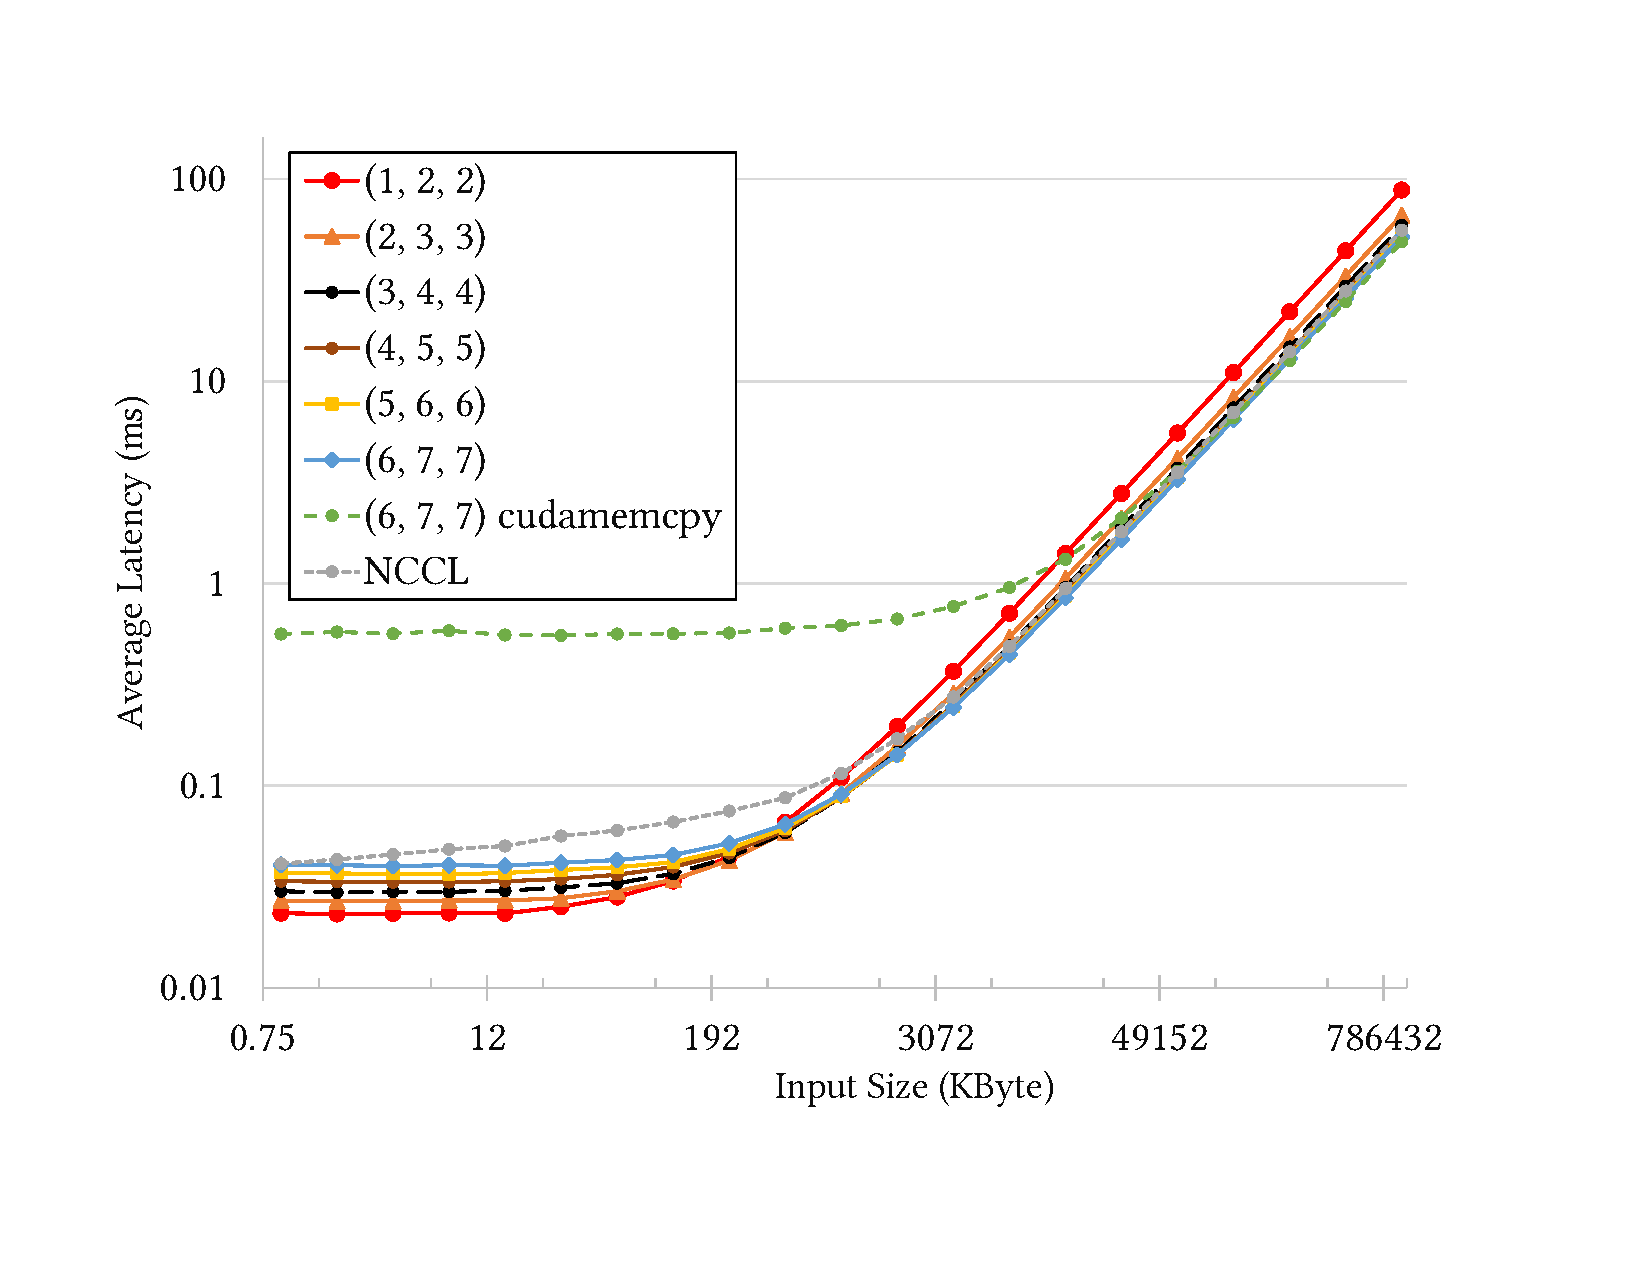
\includegraphics[page=1,width=0.84\columnwidth]{figures/evals-camera-ready}
  }
  \hfill
  \subfloat[Speedup\label{fig:dgx1-res-allgather-speedup}] {
    \includegraphics[page=2,width=0.84\columnwidth]{figures/evals-camera-ready}
  }
  \caption{\allgather performance comparison with NCCL.}
  \label{fig:dgx1-res-allgather}
\end{figure}

Figure~\ref{fig:dgx1-res-allgather} compares \tool's generated code
for \allgather with NCCL's \allgather. A point on
Figure~\ref{fig:dgx1-res-allgather-avglat} ($x$,$y$) shows the running
time in $y$ milliseconds as a function of send input buffer size in
$x$ Kbytes while a point on
Figure~\ref{fig:dgx1-res-allgather-speedup} shows the $y$ speedup of
\tool's generated code over NCCL's \allgather as a function of send
input buffer size in $x$ Kbytes. We plot one line per algorithm
denoted as $(\chunk, \steps, \rounds)$ for respectively chunks, steps,
and rounds as defined in Table~\ref{fig:dgxone:syn}. To show the
impact of our lowering, we plot two versions of a bandwidth optimal
algorithm $(6,7,7)$ (which utilizes a push-copy) and $(6,7,7)$
\texttt{cudaMemcpy}.  The latter of which shows the significant impact
lowering can have on the performance. To simplify the figure, we only
show algorithms that were faster on at least one input size we
experimented with. As it can be seen from the lines, \tool{} is up-to
$2.2\times$ faster than NCCL's \allgather on small sizes and
$1.14\times$ faster on larger sizes. It is possible for \tool{} to
automatically switch between multiple implementations based on the
input size. In which case, \tool{} will consistently outperform NCCL.

\begin{figure}[tbp]
  \centering
  \subfloat[Average latency\label{fig:dgx1-res-allreduce-avglat}] {
    \includegraphics[page=3,width=0.84\columnwidth]{figures/evals-camera-ready}
  }
  \hfill
  \subfloat[Speedup\label{fig:dgx1-res-allreduce-speedup}] {
    \includegraphics[page=4,width=0.84\columnwidth]{figures/evals-camera-ready}
  }
  \caption{\allreduce performance comparison with NCCL.}
  \label{fig:dgx1-res-allreduce}
\end{figure}


Likewise, Figure~\ref{fig:dgx1-res-allreduce} shows the running time
in milliseconds (Figure~\ref{fig:dgx1-res-allreduce-avglat}) or
speedup (Figure~\ref{fig:dgx1-res-allreduce-speedup}) for \allreduce
as a function of the receive input size.  Each line denotes $(\chunk,
\steps, \rounds)$ for respectively chunks, steps, and rounds,
respectively. With the exception of $4$ middle sizes, \tool{} beats
NCCL's \allreduce with an 8-chunk algorithm for small input sizes by
up-to $1.8\times$ and with a 48-chunk algorithm for large input sizes
by up-to $1.06\times$.

\alltoall is a complex algorithm which is very difficult to write
efficiently by hand. Unlike the prior collectives, NCCL does not
natively support \alltoall; instead, NCCL suggests using $N$
point-to-point exchanges (for $N$ GPUs) and thus its resulting
algorithm is neither bandwidth nor latency optimal.  Because \tool{}
uses program synthesis to generate optimal algorithms, it is able to
synthesize three \alltoall{} algorithms in a matter of minutes.
Figure~\ref{fig:dgx1-res-alltoall-avglat} shows the latency in
milliseconds of \tool{} and NCCL as a function of input size while
Figure~\ref{fig:dgx1-res-alltoall-speedup} shows speedup over NCCL
again as a function of input size.  Each line denotes $(\chunk,
\steps, \rounds)$ for respectively chunks, steps, and rounds and
demonstrates a speedup of over $6.8\times$ for large input sizes and
over $1.4\times$ for small input sizes, depending on whether we pick a
latency or bandwidth optimal implementation from \tool.  This
significant speedup really shows off the power of \tool's automated
approach to building algorithms tailored specifically to a hardware
architecture.

\begin{figure}[tbp]
  \centering
  \subfloat[Average latency\label{fig:dgx1-res-alltoall-avglat}]{
    \includegraphics[page=5,width=0.84\columnwidth]{figures/evals-camera-ready}
  }
  \hfill
  \subfloat[Speedup\label{fig:dgx1-res-alltoall-speedup}] {
    \includegraphics[page=6,width=0.84\columnwidth]{figures/evals-camera-ready}
  }
  \caption{\alltoall performance comparison with NCCL.}
  \label{fig:dgx1-res-alltoall}
\end{figure}

Lastly, we demonstrate \allgather on the Gigabyte AMD workstation.
Like the other plots, a point on Figure~\ref{fig:amd-res-allgather}
($x$,$y$) shows the latency or speedup $y$ for \allgather as a
function of the receive input size in bytes $x$.  We plot two
algorithms, $(1,4,4)$ and $(2,7,7)$; it is clear that (i) the lower
latency algorithm $(1,4,4)$ is better at smaller input sizes, (ii) the
higher bandwidth algorithm $(2,7,7)$ is faster for large input sizes,
and (iii) \tool's generated code is faster than RCCL for large sizes
but slower for medium and small sizes. The Gigabyte machine, in
particular, is new hardware and \tool{} can synthesize new algorithms
and implementations for it; this shows \tool{} can help design future
interconnects and co-design them with communication libraries.

These graphs in concert show that \tool{} is able to synthesize
algorithms along the Pareto-optimal frontier and also lower than to
hardware so as to be competitive with a hand optimized baseline.

\begin{figure}[tbp]
  \centering
  \subfloat[Average latency\label{fig:amd-res-allgather-avglat}]{
    \includegraphics[page=7,width=0.84\columnwidth]{figures/evals-camera-ready}
  }
  \hfill
  \subfloat[Speedup\label{fig:amd-res-allgather-speedup}] {
    \includegraphics[page=8,width=0.84\columnwidth]{figures/evals-camera-ready}
  }
  \caption{\allgather performance comparison with RCCL.}
  \label{fig:amd-res-allgather}
\end{figure}


\section{Related Work}
The message passing interface (MPI)~\cite{dongarra2013mpi} is a widely-used standardized abstraction for communication primitives in a multi processor system. Implementations of MPI provide reliable and portable implementations of collective primitives. Efficient algorithms for implementing these primitives is a long-studied research area~\cite{pjevsivac2007performance, chan2007collective, thakur2005optimization}, including optimized algorithms for specific architectures like mesh, hypercube, or fat-tree\cite{scott1991efficient,bokhari1992complete,barnett1993global} and for clusters of shared-memory processors~\cite{sistare1999optimization,traff2002improved,sanders2002hierarchical,tipparaju2003fast}. The class of $k$-synchronous algorithms studied in this paper is designed to include many of the algorithms proposed in these works and implemented in popular MPI implementations such as MPICH~\cite{thakur2005optimization} and OpenMPI~\cite{gabriel2004open}.

We evaluated OpenMPI, either through builtin CUDA capability or through Unified Communication X~(UCX)~\cite{ucx}.
They lack custom implementations for architectures such as the \dgxone{}, and result in subpar performance compared with our NCCL baselines.
NCCL~\cite{nccl} is a library for multi NVIDIA GPU systems and it utilizes the underlying hardware transport such as NVLink, NVSwitch or Infiniband for an efficient implementation of collective primitives. RCCL~\cite{rccl} is a port of NCCL for AMD GPUs and the HIP compiler suite. While these libraries provide efficient implementations for a limited set of algorithms, \tool{} is able to synthesize a wide range of algorithms suitable for different input sizes and generate collective primitives that are not even a part of standard MPI set.

There are also hybrid algorithms~\cite{barnett1994building, chan2007collective} that switch between latency- and bandwidth-optimal algorithm along each dimension of a mesh network. However, to the best of our knowledge, these prior works do not seek to identify algorithms that are Pareto-optimal for a given topology. In contrast to these prior works, the goal of this paper is to automatically synthesize Pareto-optimal algorithms for a given topology.  

There are also hierarchical approaches to implement collective primitives in distributed systems. Horovod~\cite{alex2018horovod} implements collective primitives by using NCCL locally in node and MPI across nodes. Others such as BlueConnect~\cite{blueconnect} and PLink~\cite{plink} exploit the hierarchical network topology of a cloud system or a data center to improve the performance of collective primitives. In this paper, we focus on synthesizing algorithms for a single node with multiple GPU, while the above approaches are beneficial on multi node systems.

Motivated by recent resurgence in machine-learning workloads, recent research has focused on optimizing the communication of distributed machine learning. Blink~\cite{wang2020blink}, the closest to our work, automatically synthesizes bandwidth-efficient collective primitives for a given topology. This work is based on packing spanning trees and is suitable for one-to-many collective primitives such as broadcast and reduce, and implements \allreduce as a reduce followed by a broadcast. Blink is not guaranteed to generate bandwidth-optimal algorithms as it heuristically selects a few trees based on an approximate spanning-tree packing algorithm. Moreover, Blink's focus is not on generating latency-optimal algorithms. In contrast, this work generates latency- and bandwidth-optimal algorithms for a given topology. There are also other works~\cite{zhang2017poseidon,hashemi2019tictac,jayarajan2019priority,peng2019generic} on optimizing distributed machine learning that do so by overlapping computation and communication and are orthogonal to this work. 

%\todo{Compare to related work on synthesizing compute kernels. Orthogonal.}

%\todo{Compareasd to related work on pipelining compute and communication. Orthogonal.} 

%%% Local Variables:
%%% mode: latex
%%% TeX-master: "paper"
%%% End:

\section{Conclusion}
This chapter introduces \tool: a systematic method to synthesize
algorithms in the Pareto-frontier spanning from the latency-optimal
algorithm to the bandwidth-optimal algorithm for a given collective on
an input topology. We characterize a class of algorithms that captures
a broad set of known algorithms and prove Pareto-optimality of both
known algorithms and synthesized new algorithms. We automatically
generate an implementation of these algorithms that is competitive
with manually hand-tuned communication kernels in use today.
